\documentclass[11pt, a4paper]{article}

\usepackage[utf8]{inputenc}
\usepackage[T1]{fontenc}
\usepackage[portuguese,provide=*]{babel}
\usepackage{amsmath, amssymb}
\usepackage{graphicx}
\usepackage{geometry}
\usepackage{setspace}
\usepackage[hidelinks]{hyperref}
\usepackage{xurl}
\usepackage{booktabs}
\usepackage{caption}
\usepackage{subcaption}
\usepackage{float}
\usepackage{listings}
\usepackage{xcolor}
\usepackage{enumitem}
\usepackage{array}
\usepackage{titlesec}
\titlespacing*{\section}{0pt}{7pt plus 1pt minus 1pt}{2.5pt plus 1pt minus 1pt}
\titlespacing*{\subsection}{0pt}{5pt plus 1pt minus 1pt}{2pt plus 1pt minus 1pt}
\titlespacing*{\subsubsection}{0pt}{4pt plus 1pt minus 1pt}{1pt plus 1pt minus 1pt}
\titlespacing*{\paragraph}{0pt}{2.5pt plus 1pt minus 1pt}{0.8em}
\setlist{noitemsep,topsep=2pt,parsep=1pt}

\geometry{left=1.7cm, right=1.7cm, top=1.5cm, bottom=1.5cm}
\setstretch{1.15}

\lstset{
    language=C++,
    basicstyle=\scriptsize\ttfamily,
    keywordstyle=\color{blue!80!black}\bfseries,
    commentstyle=\color{green!50!black}\itshape,
    stringstyle=\color{red!70!black},
    numbers=left,
    numberstyle=\tiny\color{gray},
    stepnumber=1,
    numbersep=4pt,
    backgroundcolor=\color{gray!6},
    frame=single,
    rulecolor=\color{gray!30},
    breaklines=true,
    tabsize=2,
    showstringspaces=false
}

\setlength{\floatsep}{5pt plus 1pt minus 1pt}
\setlength{\textfloatsep}{6pt plus 1pt minus 1pt}
\setlength{\intextsep}{5pt plus 1pt minus 1pt}
\captionsetup{font=small,labelfont=bf,skip=4pt}

\title{\textbf{Estudo Comparativo de Estruturas em Árvores Avançadas: \\ Modelagem, Análise Teórica e Avaliação Empírica}}
\author{Heitor Henrique Zonho \\ \textit{Centro Federal de Educação Tecnológica de Minas Gerais (CEFET-MG)} \\ \small Repositório: \url{https://github.com/HeitorHenriqueZ/Trabalho_Arvores}}
\date{}

\begin{document}

\maketitle

\begin{abstract}
Este trabalho apresenta uma investigação comparativa de cinco estruturas hierárquicas avançadas de dados desenvolvidas em C++17: Trie, Árvore Patricia (modelada como Radix Tree com compressão de caminhos), Árvore Splay, Treap e KD-Tree ($K=2$). Para cada estrutura, analisam-se as propriedades invariantes, a topologia e ocupação dos nós em memória, os algoritmos fundamentais de inserção, busca e remoção, além do rastreamento visual de seus estados dinâmicos. A análise assintótica contrapõe essas estruturas à Árvore Binária de Busca clássica e à Árvore AVL. A avaliação experimental afere o desempenho para cardinalidades $N \in \{10^{4}, 10^{5}, 5\cdot10^{5}\}$ sob distribuições uniforme, estritamente ordenada e com localidade de acesso temporal (80-20), correlacionando o consumo de nós e tempo de execução aos limites teóricos. Ao final, a Seção~\ref{sec:conclusao} sintetiza as conclusões fundamentadas nas questões diretivas do estudo.
\end{abstract}

\section{Introdução e Fundamentação Teórica}

Árvores Binárias de Busca (BST) e Árvores AVL organizam chaves sob ordem total unidimensional~\cite{cormen2009}. Na BST, o caso médio de busca, inserção e remoção é $O(\log n)$; com chaves ordenadas, a topologia degenera em lista linear com custo $O(n)$. A AVL impõe a invariante de equilíbrio $BF(u)=h(u.right)-h(u.left)\in\{-1,0,1\}$, limitando a altura máxima a aproximadamente $1{,}44\log_2(n+2)$ e garantindo $O(\log n)$ no pior caso~\cite{sedgewick2011} à custa de rotações e metadados de altura por nó.

Essas estruturas de busca convencionais apresentam limitações em cenários específicos:
\begin{enumerate}
    \item \textbf{Cadeias de caracteres (strings):} comparações de chaves de comprimento $m$ demandam até $O(m)$ operações, elevando o custo em BST e AVL a $O(m\log n)$;
    \item \textbf{Localidade temporal de referência:} padrões de acesso assimétricos ou concentrados (lei de Zipf / regra 80-20) não alteram a topologia de busca da AVL ou da BST estática;
    \item \textbf{Espaço multidimensional:} não existe ordenação linear natural total para tuplas ou pontos espaciais multidimensionais $(x,y,\ldots)$.
\end{enumerate}

\subsection{Invariantes das cinco estruturas}

\paragraph{Trie~\cite{fredkin1960}.}
Cada aresta corresponde a um símbolo de $\Sigma$. O caminho da raiz até o nível $d$ fixa o prefixo de tamanho $d$; um nó é terminal somente se o indicador booleano \texttt{isEndOfWord} estiver ativo.

\paragraph{Patricia~\cite{morrison1968}.}
Compactam-se caminhos unários: nós internos não terminais, salvo a raiz sentinela, têm grau $\ge 2$, e cadeias de caracteres contíguas sem bifurcação são comprimidas em uma única aresta rotulada com \texttt{prefix}. Nesta implementação, adota-se a formulação de Radix Tree / Compact Trie com rótulos de string (substrings contíguas), diferenciando-se da Patricia canônica estrita que opera com índices numéricos de desvio em nível de bits individuais (\textit{bit-skip index}). Mantém-se, contudo, a propriedade essencial de compressão de caminhos com divisão (\textit{split}) e fusão (\textit{merge}) sob demanda.

\paragraph{Splay~\cite{sleator1985}.}
BST sem metadados extras. Após acesso à chave $k$, rotações Zig / Zig-Zig / Zig-Zag levam $k$ (ou o último nó visitado) à raiz, preservando a ordem simétrica.

\paragraph{Treap~\cite{seidel1996}.}
Cada nó associa chave ordenada e prioridade aleatória (Max-Heap), satisfazendo $\mathrm{prio}(u) \ge \mathrm{prio}(u.\mathrm{left})$ e $\mathrm{prio}(u) \ge \mathrm{prio}(u.\mathrm{right})$.

\paragraph{KD-Tree~\cite{bentley1975}.}
Em profundidade $d$, o eixo é $\kappa=d\bmod K$. À esquerda, $v[\kappa]<u[\kappa]$; à direita, $w[\kappa]\ge u[\kappa]$.

\subsection{Anatomia dos nós}

\begin{table}[htbp]
\centering
\scriptsize
\resizebox{\textwidth}{!}{%
\begin{tabular}{@{}llp{5.8cm}@{}}
\toprule
\textbf{Estrutura} & \textbf{Campos} & \textbf{Organização} \\ \midrule
Trie & \texttt{children[256]}, \texttt{isEndOfWord} & 256 ponteiros por nó ($\approx$2048\,B em 64 bits) \\
Patricia & \texttt{prefix}, \texttt{children}, flag & \texttt{string}+\texttt{vector}; alocação sob demanda \\
Splay & \texttt{key}, \texttt{left}, \texttt{right} & Sem altura/cor; $\approx$24\,B/nó \\
Treap & campos da Splay + \texttt{priority} & 24\,B no ABI x86\_64 verificado (usa padding) \\
KD-Tree & \texttt{coords[K]}, \texttt{left}, \texttt{right} & $K=2$: duas coordenadas inteiras \\
\bottomrule
\end{tabular}}
\caption{Anatomia dos nós (arquitetura 64 bits).}
\label{tab:anatomia_nos}
\end{table}

\section{Projeto e Implementação das Estruturas}

Implementação em ISO C++17, com cabeçalhos em \texttt{include/} e fontes em \texttt{src/}. Cópia e movimentação das classes foram desabilitadas (\texttt{= delete}) para evitar double-free. Duplicatas são rejeitadas na Splay, Treap e KD-Tree; em Trie/Patricia a reinscrição apenas reativa o marcador terminal.

\subsection{Memória e build}

Com o intuito de mitigar riscos de esgotamento de pilha (\textit{stack overflow}) decorrentes de recursão profunda durante a desalocação de árvores severamente desbalanceadas em cargas elevadas ($N = 500.000$), os destrutores das árvores binárias (Splay, Treap e KD-Tree) foram implementados mediante desalocação iterativa com rotações de cauda (padrão Day-Stout-Warren), assegurando consumo auxiliar de espaço $O(1)$. Todas as estruturas implementam semântica estrita de gerenciamento de recursos (RAII), com cópias e movimentações explicitamente suprimidas (\texttt{= delete}) para impedir cópias rasas acidentais e liberação dupla (\textit{double-free}). O projeto adota compilação limpa sob \texttt{-std=c++17 -Wall -Wextra -pedantic} no GCC, com testes automatizados em \texttt{tests/test\_trees.cpp} e verificação contínua de vazamento de memória via AddressSanitizer (\texttt{make asan}). O código-fonte integral encontra-se referenciado no repositório oficial do projeto.

\subsection{Operações}

\subsubsection{Trie}
Inserção aloca filhos sob demanda e marca o terminal. Remoção desmarca e apaga nós sem filhos no retorno da recursão.

\subsubsection{Patricia}
Se o prefixo comum $L$ for estritamente menor que $|u.\mathrm{prefix}|$, ocorre \textit{split} (Listagem~\ref{lst:patricia_split}). Na remoção, nós não terminais com um único filho são fundidos.

\begin{lstlisting}[caption={Split na Patricia},label={lst:patricia_split}]
int L = commonPrefixLength(child->prefix, word);
if (L > 0 && L < (int)child->prefix.length()) {
    PatriciaNode* split = new PatriciaNode(child->prefix.substr(L));
    split->children = child->children; split->isEndOfWord = child->isEndOfWord;
    child->prefix = child->prefix.substr(0, L); child->children = { split };
    child->isEndOfWord = (L == (int)word.length());
    if (!child->isEndOfWord) {
        PatriciaNode* novo = new PatriciaNode(word.substr(L));
        novo->isEndOfWord = true; child->children.push_back(novo);
    }
}
\end{lstlisting}

\subsubsection{Splay}
\texttt{splay(root,key)} aplica recursivamente Zig-Zig/Zig-Zag. Na remoção, a chave sobe à raiz; as subárvores são reunidas pelo máximo da esquerda.

\subsubsection{Treap}
Inserção BST com rotações na volta para restaurar o Max-Heap (Algoritmo~\ref{alg:treap}). Remoção rotaciona o alvo até haver no máximo um filho, que o substitui. Prioridades usam \texttt{std::mt19937}.

\begin{lstlisting}[caption={Inserção na Treap (Max-Heap)},label={alg:treap}]
Insert(node, key, priority):
    if node == null: return new Node(key, priority)
    if key == node.key: return node
    if key < node.key:
        node.left = Insert(node.left, key, priority)
        if node.left.priority > node.priority:
            node = RightRotate(node)
    else:
        node.right = Insert(node.right, key, priority)
        if node.right.priority > node.priority:
            node = LeftRotate(node)
    return node
\end{lstlisting}

\subsubsection{KD-Tree (K = 2)}
Comparação em $cd=\mathrm{depth}\bmod 2$. Remoção (Algoritmo~\ref{alg:kdtree_remove}): substitui pelo mínimo na dimensão $cd$ da subárvore direita; se só houver esquerda, move-a para a direita antes de remover o substituto.

\begin{lstlisting}[caption={Remoção na KD-Tree},label={alg:kdtree_remove}]
RemoveHelper(root, pt, depth):
    if root == null: return null
    cd = depth % 2
    if root.point == pt:
        if root.right != null:
            min = FindMin(root.right, cd, depth + 1)
            root.point = min.point
            root.right = RemoveHelper(root.right, min.point, depth + 1)
        else if root.left != null:
            min = FindMin(root.left, cd, depth + 1)
            root.point = min.point
            root.right = RemoveHelper(root.left, min.point, depth + 1)
            root.left = null
        else:
            delete root
            return null
        return root
    if pt[cd] < root.point[cd]:
        root.left = RemoveHelper(root.left, pt, depth + 1)
    else:
        root.right = RemoveHelper(root.right, pt, depth + 1)
    return root
\end{lstlisting}

\paragraph{Vizinho Mais Próximo (Nearest Neighbor).}
A operação \texttt{nearestNeighbor} percorre a árvore de forma recursiva, mantendo o melhor candidato encontrado e podando subárvores cujo hiperplano separador está mais distante do que a melhor distância corrente. A cada nível, o algoritmo visita primeiro o lado do espaço que contém o ponto alvo, atualizando a distância mínima, e só explora o outro lado se a distância ao hiperplano ($|\mathrm{target}[cd] - \mathrm{node}[cd]|^2$) for inferior à melhor distância conhecida. Em baixa dimensão e sob distribuição favorável, o custo esperado é $O(\log n)$; o pior caso é $O(n)$.

\paragraph{Busca por Faixa (Range Search).}
A operação \texttt{rangeSearch} retorna todos os pontos contidos em um retângulo ortogonal $[\mathrm{low}, \mathrm{high}]$. Em cada nó, o algoritmo verifica se o ponto pertence à faixa e, pelo eixo discriminante $cd$, poda subárvores que não podem interceptar o retângulo: a subárvore esquerda é visitada apenas se $\mathrm{low}[cd] \le \mathrm{node}[cd]$, e a direita apenas se $\mathrm{high}[cd] \ge \mathrm{node}[cd]$. Em uma árvore balanceada, a complexidade para $K=2$ é $O(\sqrt{n} + k)$, onde $k$ é o número de pontos reportados.

\section{Demonstração e Rastreamento Visual}

Para cada estrutura: (1) estado após inserções iniciais; (2) estado intermediário com o mecanismo típico; (3) estado após remoção. As quinze imagens desta seção foram geradas diretamente pelos métodos \texttt{toDot()} das cinco classes, por meio de \texttt{make diagrams}; os arquivos DOT também acompanham o código. Nós terminais de Trie e Patricia aparecem destacados, e os pequenos pontos pretos nas árvores binárias representam filhos nulos.

\subsection{Trie}
Figura~\ref{fig:trace_trie}: (a) ``roma''; (b) ``romano'' reutiliza o prefixo; (c) remoção de ``roma'' desativa o terminal em ``a''.

\begin{figure}[H]
    \centering
    \begin{subfigure}[b]{0.31\textwidth}
        \centering
        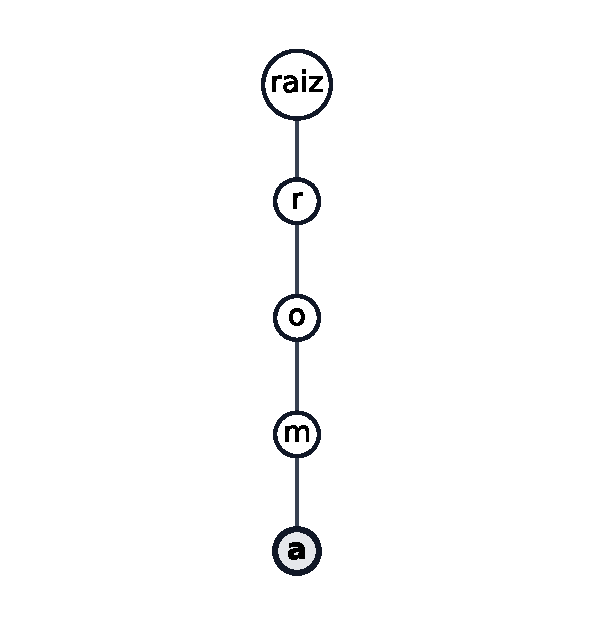
\includegraphics[width=\linewidth,height=5.0cm,keepaspectratio]{diagramas/trie_1.pdf}
        \caption{Inicial: ``roma''}
    \end{subfigure}
    \hfill
    \begin{subfigure}[b]{0.33\textwidth}
        \centering
        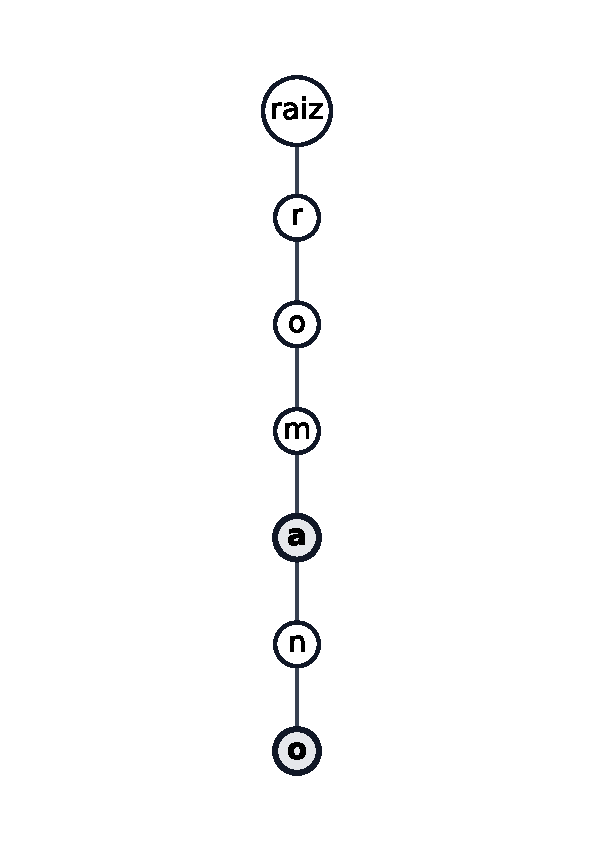
\includegraphics[width=\linewidth,height=5.0cm,keepaspectratio]{diagramas/trie_2.pdf}
        \caption{Intermediário: ``romano''}
    \end{subfigure}
    \hfill
    \begin{subfigure}[b]{0.33\textwidth}
        \centering
        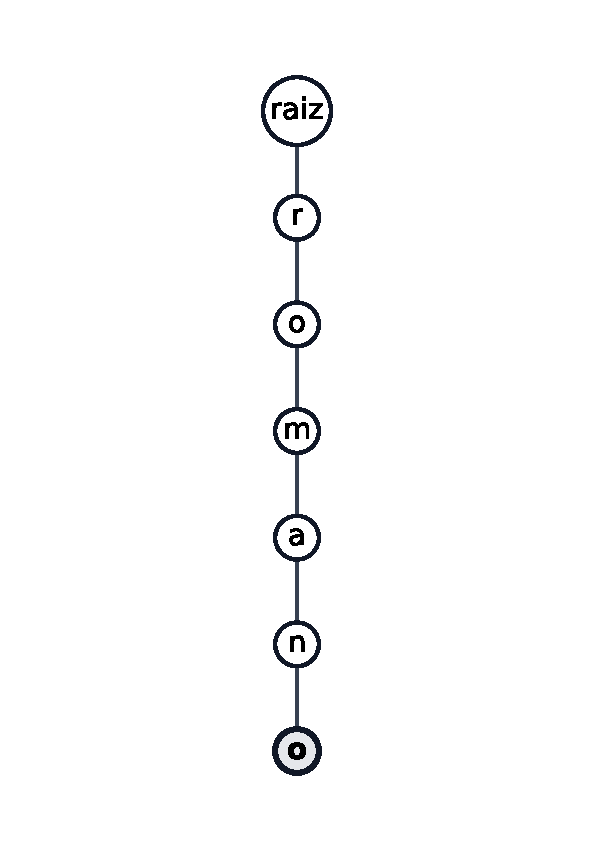
\includegraphics[width=\linewidth,height=5.0cm,keepaspectratio]{diagramas/trie_3.pdf}
        \caption{Pós-remoção ``roma''}
    \end{subfigure}
    \caption{Trie: compartilhamento de prefixos.}
    \label{fig:trace_trie}
\end{figure}

\subsection{Patricia}
Figura~\ref{fig:trace_patricia}: (a) ``roma''/``romano''; (b) split com ``rato''; (c) remoção de ``romano''.

\begin{figure}[H]
    \centering
    \begin{subfigure}[b]{0.28\textwidth}
        \centering
        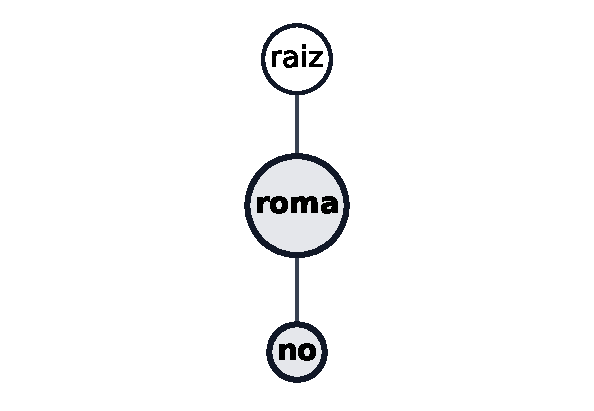
\includegraphics[width=\linewidth,height=4.8cm,keepaspectratio]{diagramas/patricia_1.pdf}
        \caption{Inicial}
    \end{subfigure}
    \hfill
    \begin{subfigure}[b]{0.34\textwidth}
        \centering
        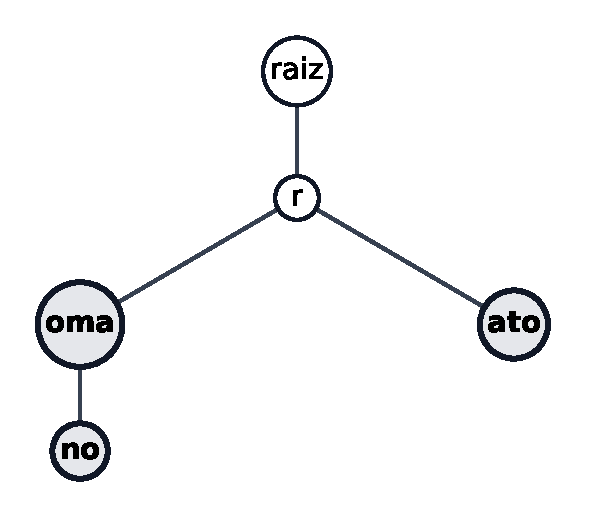
\includegraphics[width=\linewidth,height=4.8cm,keepaspectratio]{diagramas/patricia_2.pdf}
        \caption{Split com ``rato''}
    \end{subfigure}
    \hfill
    \begin{subfigure}[b]{0.34\textwidth}
        \centering
        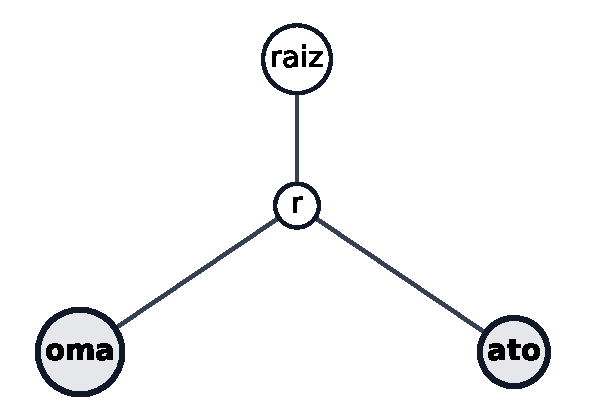
\includegraphics[width=\linewidth,height=4.8cm,keepaspectratio]{diagramas/patricia_3.pdf}
        \caption{Pós-remoção ``romano''}
    \end{subfigure}
    \caption{Patricia: compressão e split.}
    \label{fig:trace_patricia}
\end{figure}

\subsection{Splay}
Figura~\ref{fig:trace_splay}: inserção ordenada 10--20--30 com splay ativo (cada inserção eleva o novo nó à raiz); busca de 10 via \texttt{search(10)}; remoção de 20. Estados verificados via \texttt{toDot()}.

\begin{figure}[H]
    \centering
    \begin{subfigure}[b]{0.31\textwidth}
        \centering
        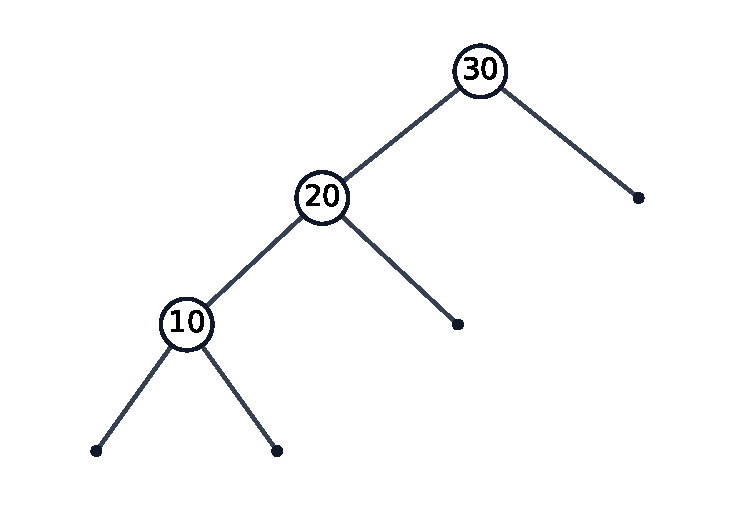
\includegraphics[width=\linewidth,height=4.8cm,keepaspectratio]{diagramas/splay_1.pdf}
        \caption{Após insert(10,20,30)}
    \end{subfigure}
    \hfill
    \begin{subfigure}[b]{0.31\textwidth}
        \centering
        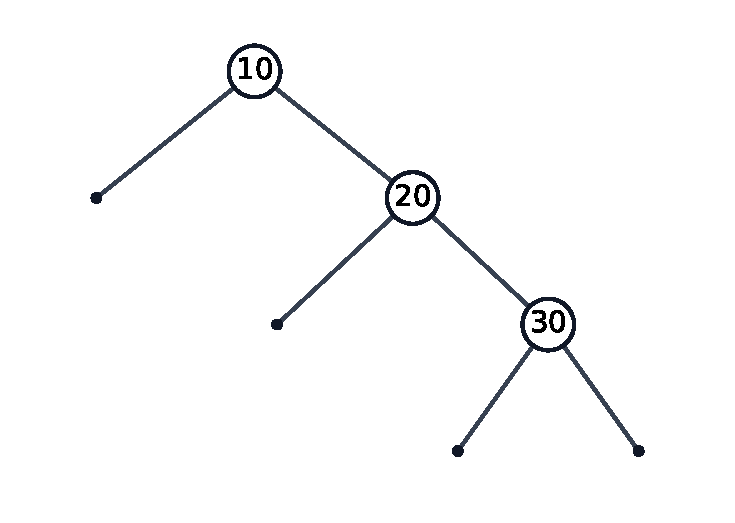
\includegraphics[width=\linewidth,height=4.8cm,keepaspectratio]{diagramas/splay_2.pdf}
        \caption{Após search(10)}
    \end{subfigure}
    \hfill
    \begin{subfigure}[b]{0.31\textwidth}
        \centering
        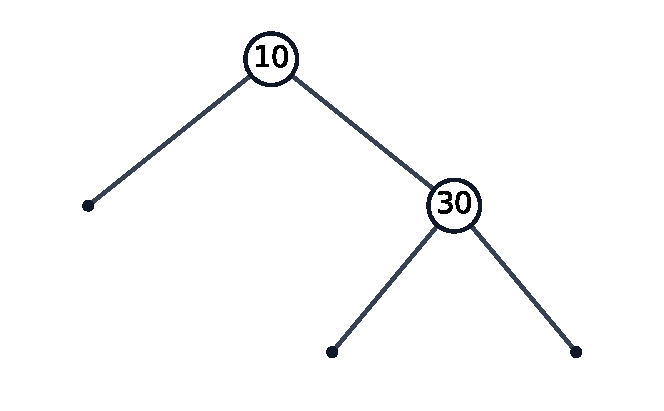
\includegraphics[width=\linewidth,height=4.8cm,keepaspectratio]{diagramas/splay_3.pdf}
        \caption{Pós-remoção(20)}
    \end{subfigure}
    \caption{Splay: auto-organização por rotação.}
    \label{fig:trace_splay}
\end{figure}

\clearpage
\subsection{Treap}
Figura~\ref{fig:trace_treap}: (a) após inserir 50; (b) inserções de 30 e 40 com prioridades reproduzíveis a partir da semente 42, acompanhadas das rotações de Max-Heap; (c) remoção da raiz 40.

\begin{figure}[H]
    \centering
    \begin{subfigure}[b]{0.31\textwidth}
        \centering
        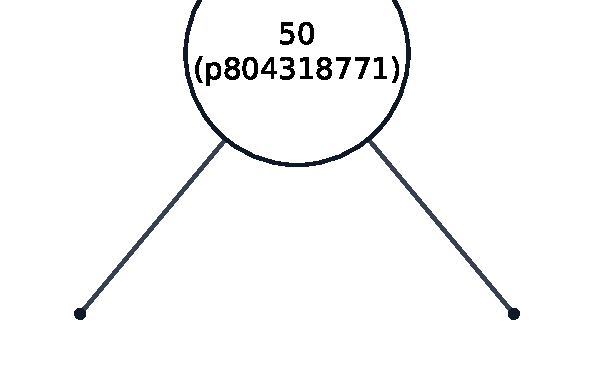
\includegraphics[width=\linewidth,height=5.0cm,keepaspectratio]{diagramas/treap_1.pdf}
        \caption{Inicial: inserção de 50}
    \end{subfigure}
    \hfill
    \begin{subfigure}[b]{0.33\textwidth}
        \centering
        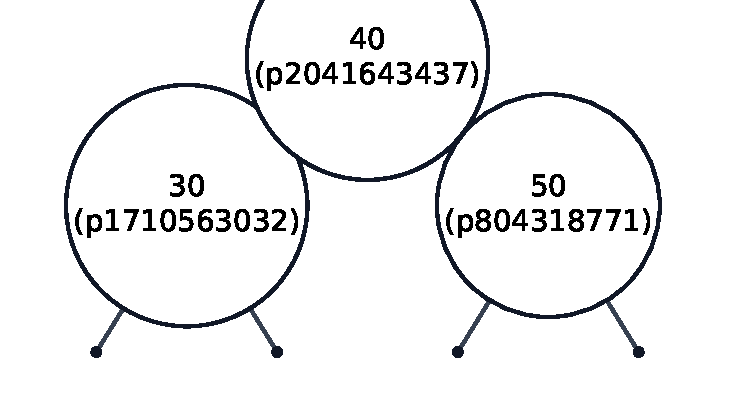
\includegraphics[width=\linewidth,height=5.0cm,keepaspectratio]{diagramas/treap_2.pdf}
        \caption{Após inserções 30 e 40}
    \end{subfigure}
    \hfill
    \begin{subfigure}[b]{0.31\textwidth}
        \centering
        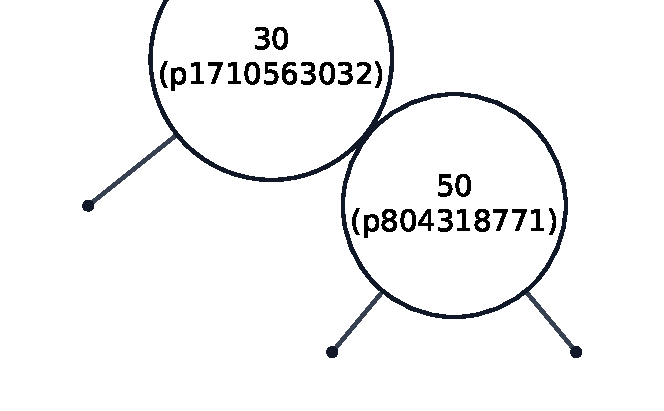
\includegraphics[width=\linewidth,height=5.0cm,keepaspectratio]{diagramas/treap_3.pdf}
        \caption{Pós-remoção da raiz 40}
    \end{subfigure}
    \caption{Treap: BST + Max-Heap.}
    \label{fig:trace_treap}
\end{figure}

\subsection{KD-Tree (K = 2)}
A Figura~\ref{fig:trace_kdtree} ilustra o particionamento bidimensional com cortes ortogonais alternados e a operação de remoção estrutural: (a) estado inicial com a raiz $(3,6)$ particionando no eixo $x=3$ e o nó $(17,15)$ em sua subárvore direita particionando no eixo $y=15$; (b) estado intermediário após a inserção de $(13,15)$, que desce pela subárvore direita da raiz ($13 \ge 3$) e pela subárvore direita de $(17,15)$ ($15 \ge 15$), assumindo corte no eixo $x=13$; (c) estado pós-remoção da raiz $(3,6)$, onde o nó substituto é o mínimo na dimensão de corte $x$ localizado na subárvore direita, correspondente a $(13,15)$, preservando as invariantes de partição espacial.

\begin{figure}[H]
    \centering
    \begin{subfigure}[b]{0.31\textwidth}
        \centering
        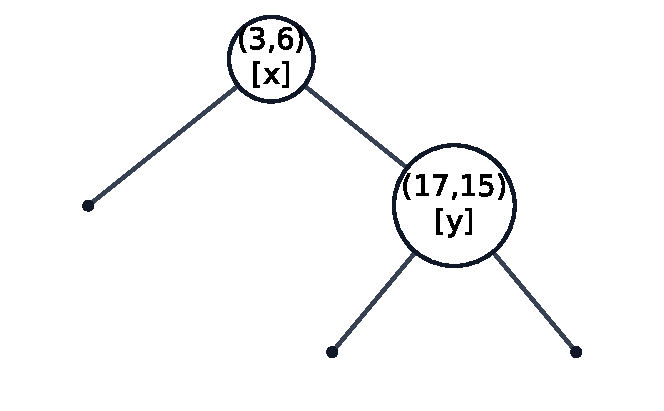
\includegraphics[width=\linewidth,height=5.0cm,keepaspectratio]{diagramas/kdtree_1.pdf}
        \caption{Inicial}
    \end{subfigure}
    \hfill
    \begin{subfigure}[b]{0.33\textwidth}
        \centering
        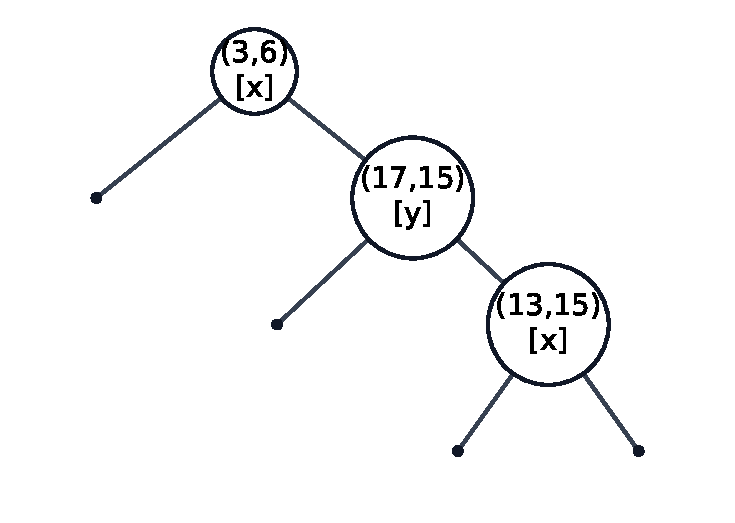
\includegraphics[width=\linewidth,height=5.0cm,keepaspectratio]{diagramas/kdtree_2.pdf}
        \caption{ins(13,15)}
    \end{subfigure}
    \hfill
    \begin{subfigure}[b]{0.31\textwidth}
        \centering
        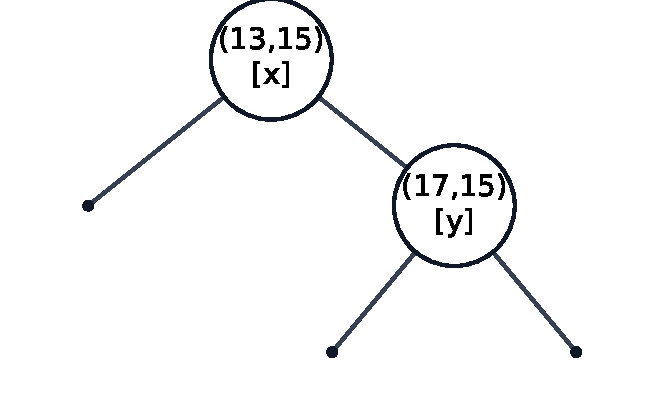
\includegraphics[width=\linewidth,height=5.0cm,keepaspectratio]{diagramas/kdtree_3.pdf}
        \caption{Pós-remoção da raiz}
    \end{subfigure}
    \caption{KD-Tree: particionamento ortogonal.}
    \label{fig:trace_kdtree}
\end{figure}

\section{Análise de Complexidade e Comparação Teórica}

A Tabela~\ref{tab:complexidade} compara as cinco estruturas com BST e AVL. Para Trie/Patricia, $m$ é o comprimento da chave (máximo na construção) e $|\Sigma|=256$. B/I/R: busca, inserção e remoção. A coluna melhor refere-se à busca; o caso médio depende da distribuição. Range pressupõe balanceamento e inclui a saída $k$.

\begin{table}[htbp]
\centering
\scriptsize
\resizebox{\textwidth}{!}{%
\begin{tabular}{@{}lcccccc@{}}
\toprule
\textbf{Estrutura} & \textbf{Melhor} & \textbf{Médio B/I/R} & \textbf{Pior B/I/R} & \textbf{Construção} & \textbf{Espaço} & \textbf{Extra} \\ \midrule
Trie & $\Theta(1)$ & $\Theta(m)$ & $O(m)$ & $O(Nm)$ & $O(Nm|\Sigma|)$ & Prefixo $O(m)$ \\
Patricia & $\Theta(1)$ & ver texto & $O(m^2)$ & $O(Nm^2)$ pior & $O(Nm)$ & Split local $O(m)$ \\
Splay & $\Theta(1)$ & $O(\log n)^{\dagger}$ & $O(n)$ & $O(N\log N)^{\dagger}$ & $O(n)$ & Amortizado \\
Treap & $\Theta(1)$ & $O(\log n)$ esp. & $O(n)$ & $O(N\log N)$ esp. / $O(N^2)$ pior & $O(n)$ & Rotação $O(1)$ \\
KD-Tree & $\Theta(1)$ & B/I: $O(\log n)$; R: texto & $O(n)$ & $O(N\log N)$ méd. / $O(N^2)$ pior & $O(n)$ & Range $O(\sqrt{n}+k)$ \\ \midrule
BST & $\Theta(1)$ & $O(\log n)$ & $O(n)$ & $O(N\log N)$ méd. / $O(N^{2})$ pior & $O(n)$ & --- \\
AVL & $\Theta(1)$ & $O(\log n)$ & $O(\log n)$ & $O(N\log N)$ & $O(n)$ & Altura $O(\log n)$ \\
\bottomrule
\multicolumn{7}{l}{\tiny $^{\dagger}$ Média amortizada (potencial de Sleator--Tarjan).}
\end{tabular}}
\caption{Complexidade assintótica frente a BST e AVL.}
\label{tab:complexidade}
\end{table}

\paragraph{Árvore Binária de Busca (BST) vs. Árvore AVL.}
Em uma BST estática, a topologia é inteiramente governada pela ordem de chegada das chaves. Sob sequências estritamente ordenadas, cada nova chave é inserida na extremidade da cadeia, degenerando a árvore em uma lista unária de altura $h = n-1$. Nessa condição, busca, inserção e remoção degradam para $\Theta(n)$ e a construção total consome $\sum_{i=1}^{n} i = \Theta(n^2)$. A Árvore AVL contrapõe essa patologia impondo a invariante de altura $|h(u.\mathrm{right}) - h(u.\mathrm{left})| \le 1$. Uma árvore AVL de altura $h$ com cardinalidade mínima obedece à recorrência de Fibonacci $N(h) = N(h-1) + N(h-2) + 1$, cuja solução analítica prova que $h < 1{,}4404\log_2(n+2) - 0{,}328$. Essa cota estrita garante complexidade $O(\log n)$ no pior caso para todas as operações fundamentais, demandando no máximo duas rotações por inserção e $O(\log n)$ rotações por remoção.

\paragraph{Árvore Splay.}
A Árvore Splay dispensa metadados de balanceamento e reorganiza a árvore após os acessos. Uma operação individual pode custar $O(n)$; as rotações não reduzem a profundidade de todos os nós visitados. A garantia é amortizada: usando $r(x)=\log_2 s(x)$ e $\Phi(T)=\sum_x r(x)$, com $s(x)$ igual ao tamanho da subárvore, o lema de acesso limita o custo amortizado do splay por $3(r(t)-r(x))+1$, onde $t$ é a raiz anterior. Assim, uma sequência de $M$ operações iniciada com árvore vazia e no máximo $n$ chaves custa $O(M\log(n+1))$. Optimalidade estática e o teorema do conjunto de trabalho são resultados adicionais sobre padrões de acesso~\cite{sleator1985}.

\paragraph{Árvore Treap.}
A Treap combina a invariante simétrica da BST para as chaves com a ordenação de Max-Heap para prioridades inteiras pseudoaleatórias, geradas em um intervalo amplo no instante de inserção. No modelo teórico de prioridades independentes e distintas, sua ordenação induz a mesma distribuição de formas de uma BST construída por permutação aleatória. No código, as prioridades são inteiras e podem empatar; as comparações estritas preservam o Max-Heap não estrito, sem assegurar identidade exata com o modelo sem empates. Pela análise clássica de árvores aleatórias, a profundidade esperada é $O(\log n)$, assegurando custo esperado $O(\log n)$ para busca, inserção e remoção, embora o pior caso permaneça $O(n)$.

\paragraph{Trie vs. Árvore Patricia.}
A Trie realiza busca, inserção e remoção em $O(m)$ para alfabeto fixo; uma busca bem-sucedida percorre $\Theta(m)$ símbolos. A Radix Tree permite $O(m)$ quando evita copiar os sufixos. Nesta Patricia, porém, cada chamada a \texttt{substr} copia a parte restante da chave: em cadeias como ``a'', ``aa'', ``aaa'', as cópias somam $m+(m-1)+\cdots+1=O(m^2)$. Esse é o pior caso das operações implementadas; o custo médio depende dos prefixos compartilhados. A construção por $N$ inserções tem cota $O(Nm^2)$. A Trie ocupa $O(Nm|\Sigma|)$; a Patricia, $O(Nm)$ em armazenamento permanente. Fora a raiz sentinela, nós não terminais têm ao menos dois filhos, limitando o total a $2N$ nós para $N\ge1$ (a árvore vazia mantém a raiz). As cópias recursivas de sufixos podem consumir ainda $O(m^2)$ de espaço temporário.

\paragraph{KD-Tree ($K=2$).}
Ao estender a partição binária para espaços multidimensionais euclidianos, a KD-Tree discrimina coordenadas alternando o hiperplano separador $\kappa = d \bmod K$ na profundidade $d$. A busca pontual exata em conjuntos aleatórios aproximadamente balanceados atinge tempo médio $O(\log n)$, enquanto operações avançadas como \texttt{nearestNeighbor} e \texttt{rangeSearch} exploram a poda de ramos espaciais. Para uma KD-Tree balanceada em duas dimensões, a consulta ortogonal tem cota típica $O(\sqrt{n}+k)$, onde $k$ é a saída; sem balanceamento, busca, remoção, vizinho mais próximo e consulta por faixa podem degradar a $O(n)$. A remoção inclui \texttt{findMin}, que pode visitar $O(\sqrt{s})$ nós em uma subárvore 2D balanceada de tamanho $s$, pois explora ambos os ramos em eixos alternados. Assim, remover um nó próximo à raiz pode custar $O(\sqrt{n})$ mesmo com balanceamento; não se atribui custo médio logarítmico à remoção sem definir a distribuição dos alvos.

\section{Metodologia Experimental e Resultados}

\subsection{Ambiente e método}
Ubuntu 24.04 LTS (Linux x86\_64, Kernel 6.6), processador Intel\textsuperscript{\textregistered} Core\texttrademark\ i3-9100F (4 núcleos / 4 threads, 3{,}60\,GHz), 16\,GB de RAM em canal único, GPU NVIDIA GeForce GTX 1050 Ti e compilador \texttt{g++} 13.3.0 (C++17, \texttt{-O3}). A GPU não participa dos cálculos. Tempos aferidos via \texttt{std::chrono::}\allowbreak\texttt{steady\_clock}, com I/O fora da região medida e semente fixa \texttt{mt19937(42)}. Cargas sintéticas sem duplicatas: strings ASCII (5--14 caracteres), inteiros em $[1, 10^{7}]$ e pontos bidimensionais em $[0, 10^{6}]^{2}$. Cada valor registrado corresponde a uma execução controlada; por isso, diferenças inferiores a 1\,ms devem ser interpretadas como abaixo da resolução adotada, e as conclusões privilegiam tendências de escala. Dados brutos registrados em \texttt{data/}.

\subsection{Tempos medidos}
Valores da Tabela~\ref{tab:dados_benchmark} são cópia direta do CSV gerado nesta máquina.

\begin{table}[htbp]
\centering
\small
\begin{tabular}{@{}lcrrr@{}}
\toprule
\textbf{Estrutura} & \textbf{$N$} & \textbf{Inserção (ms)} & \textbf{Busca (ms)} & \textbf{Remoção (ms)} \\ \midrule
Trie & $10^{4}$ & 125 & 1 & 27 \\
Patricia & $10^{4}$ & 3 & 1 & 1 \\
Splay & $10^{4}$ & 1 & 1 & 1 \\
Treap & $10^{4}$ & 1 & 0 & 1 \\
KD-Tree & $10^{4}$ & 1 & 0 & 1 \\ \midrule
Trie & $10^{5}$ & 1339 & 23 & 282 \\
Patricia & $10^{5}$ & 46 & 34 & 32 \\
Splay & $10^{5}$ & 31 & 24 & 27 \\
Treap & $10^{5}$ & 26 & 15 & 21 \\
KD-Tree & $10^{5}$ & 23 & 18 & 26 \\ \midrule
Trie & $5\cdot10^{5}$ & 5039 & 131 & 1415 \\
Patricia & $5\cdot10^{5}$ & 343 & 333 & 376 \\
Splay & $5\cdot10^{5}$ & 325 & 305 & 287 \\
Treap & $5\cdot10^{5}$ & 273 & 229 & 235 \\
KD-Tree & $5\cdot10^{5}$ & 224 & 179 & 287 \\
\bottomrule
\end{tabular}
\caption{Tempos de \texttt{benchmark\_results.csv} (ms).}
\label{tab:dados_benchmark}
\end{table}

\begin{figure}[H]
    \centering
    \begin{subfigure}[b]{0.49\textwidth}
        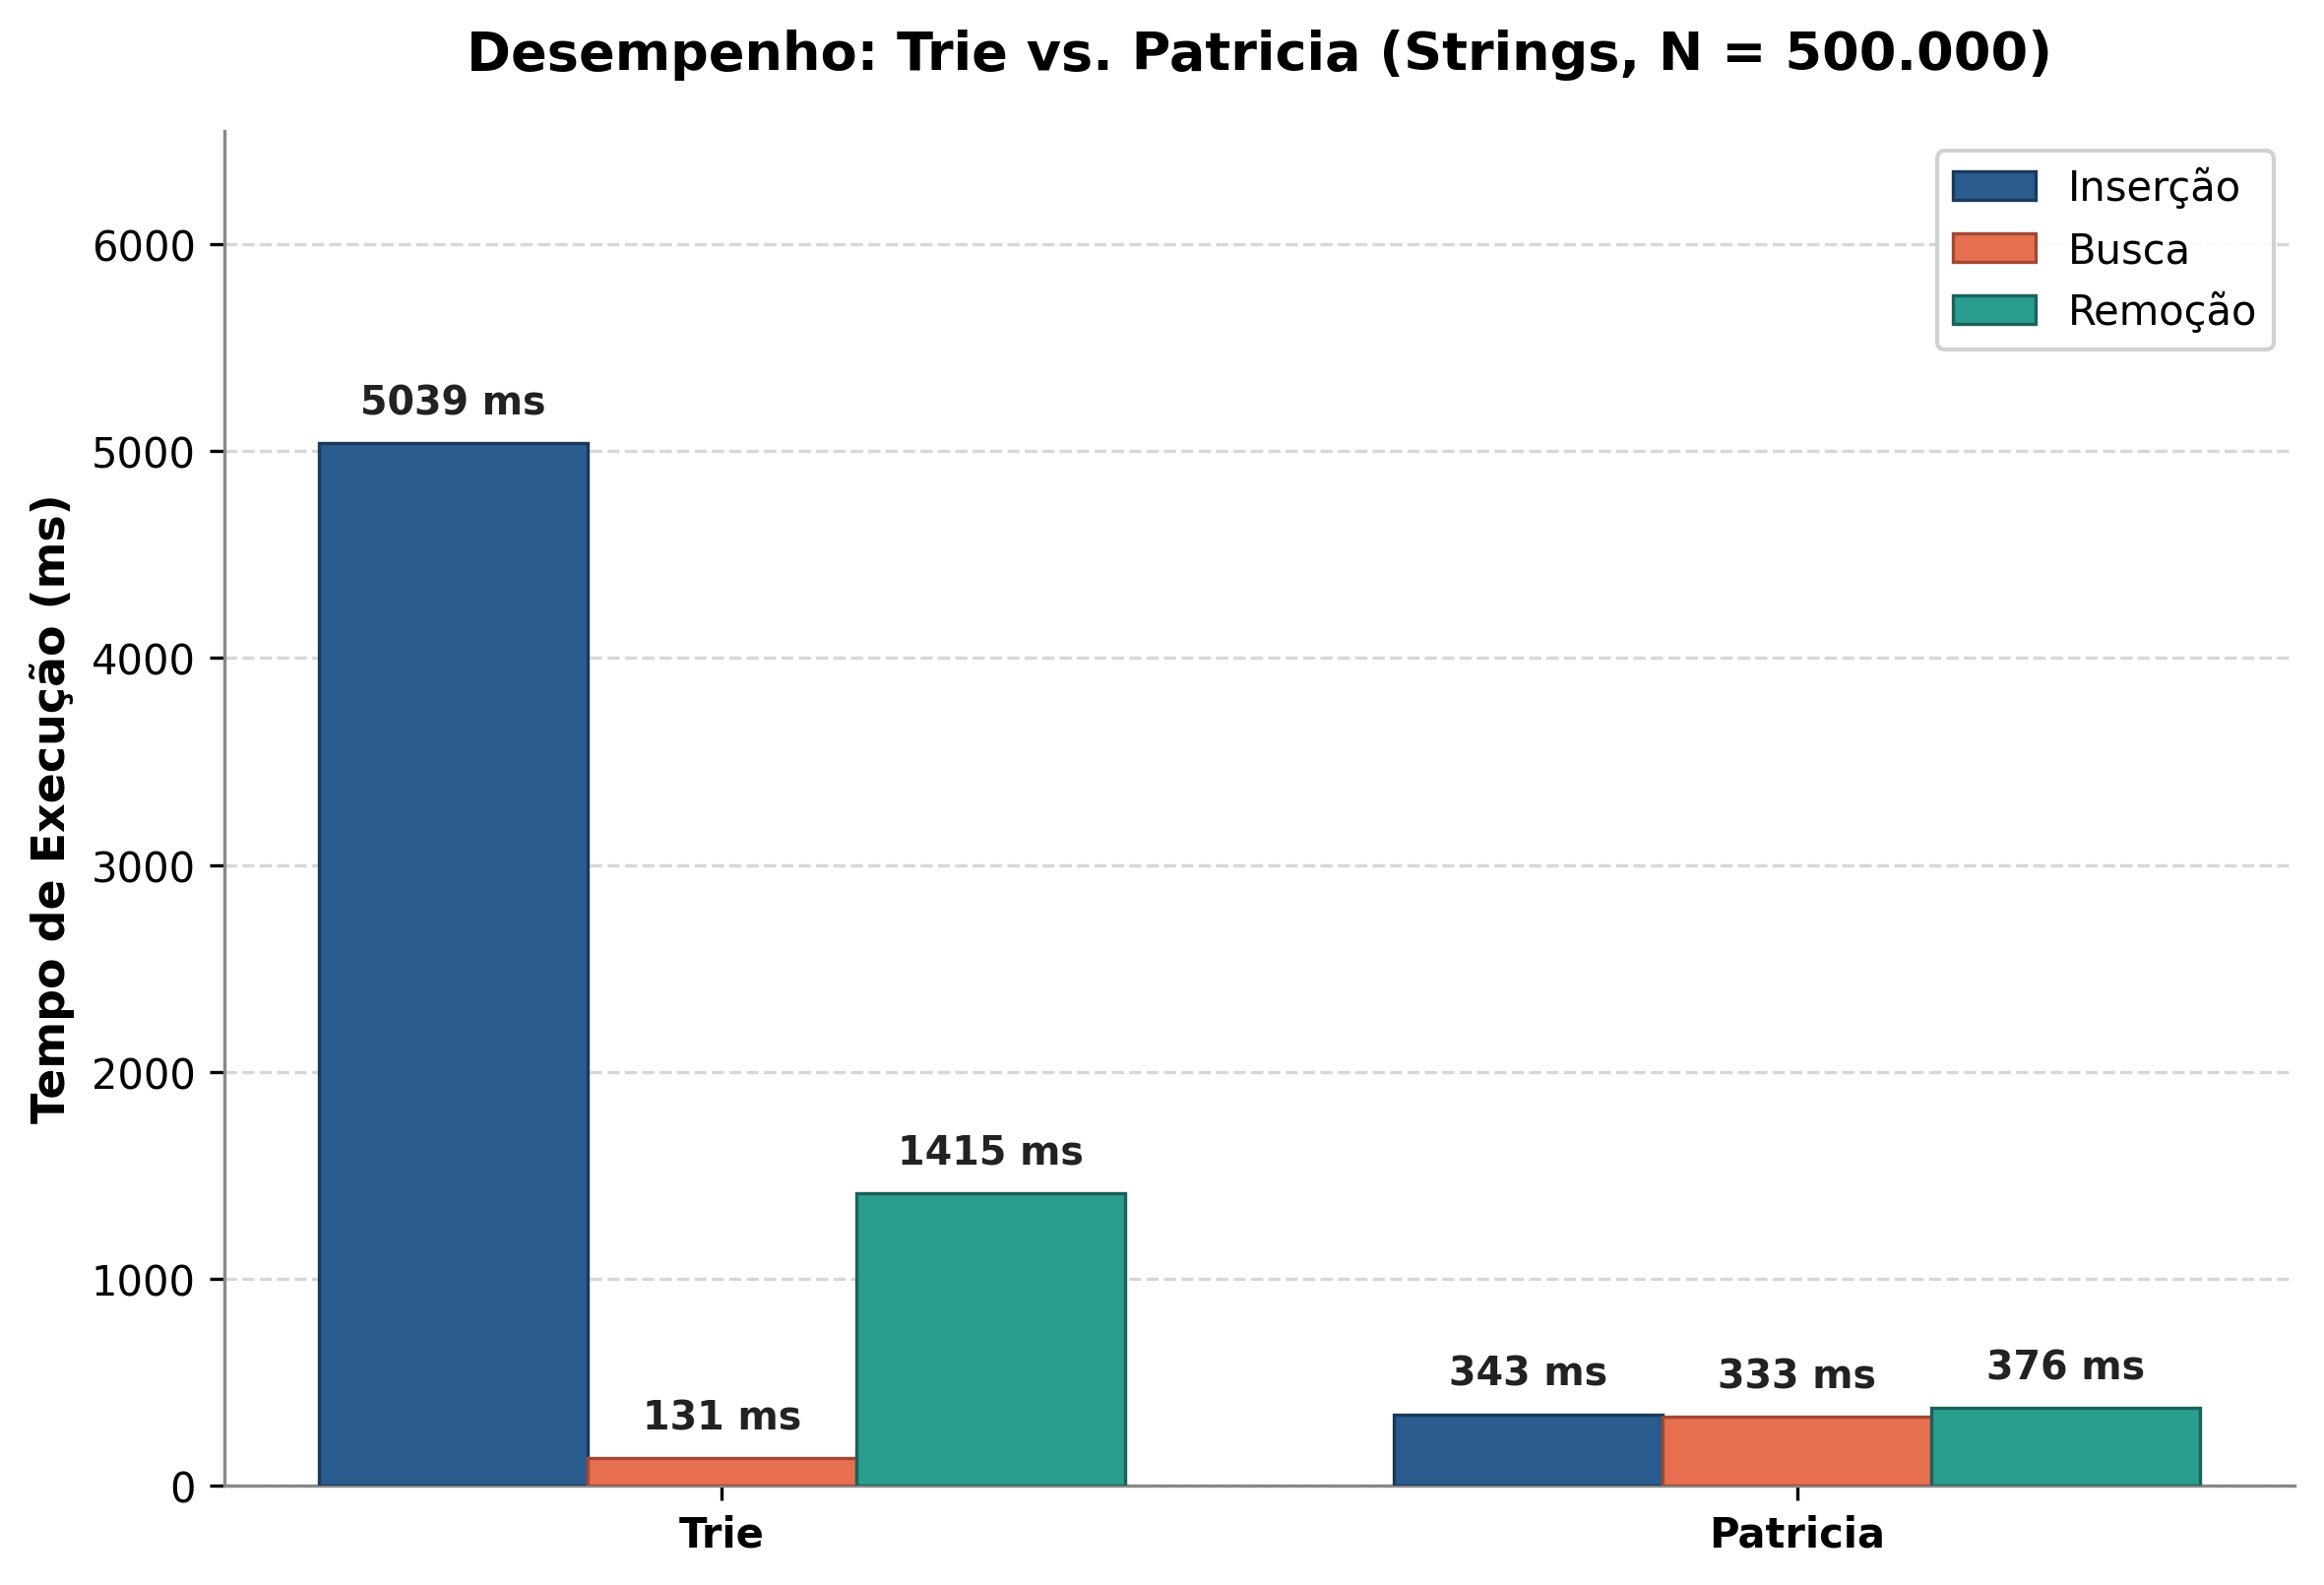
\includegraphics[width=\textwidth]{graficos/benchmark_strings.png}
        \caption{Trie vs Patricia}
    \end{subfigure}
    \hfill
    \begin{subfigure}[b]{0.49\textwidth}
        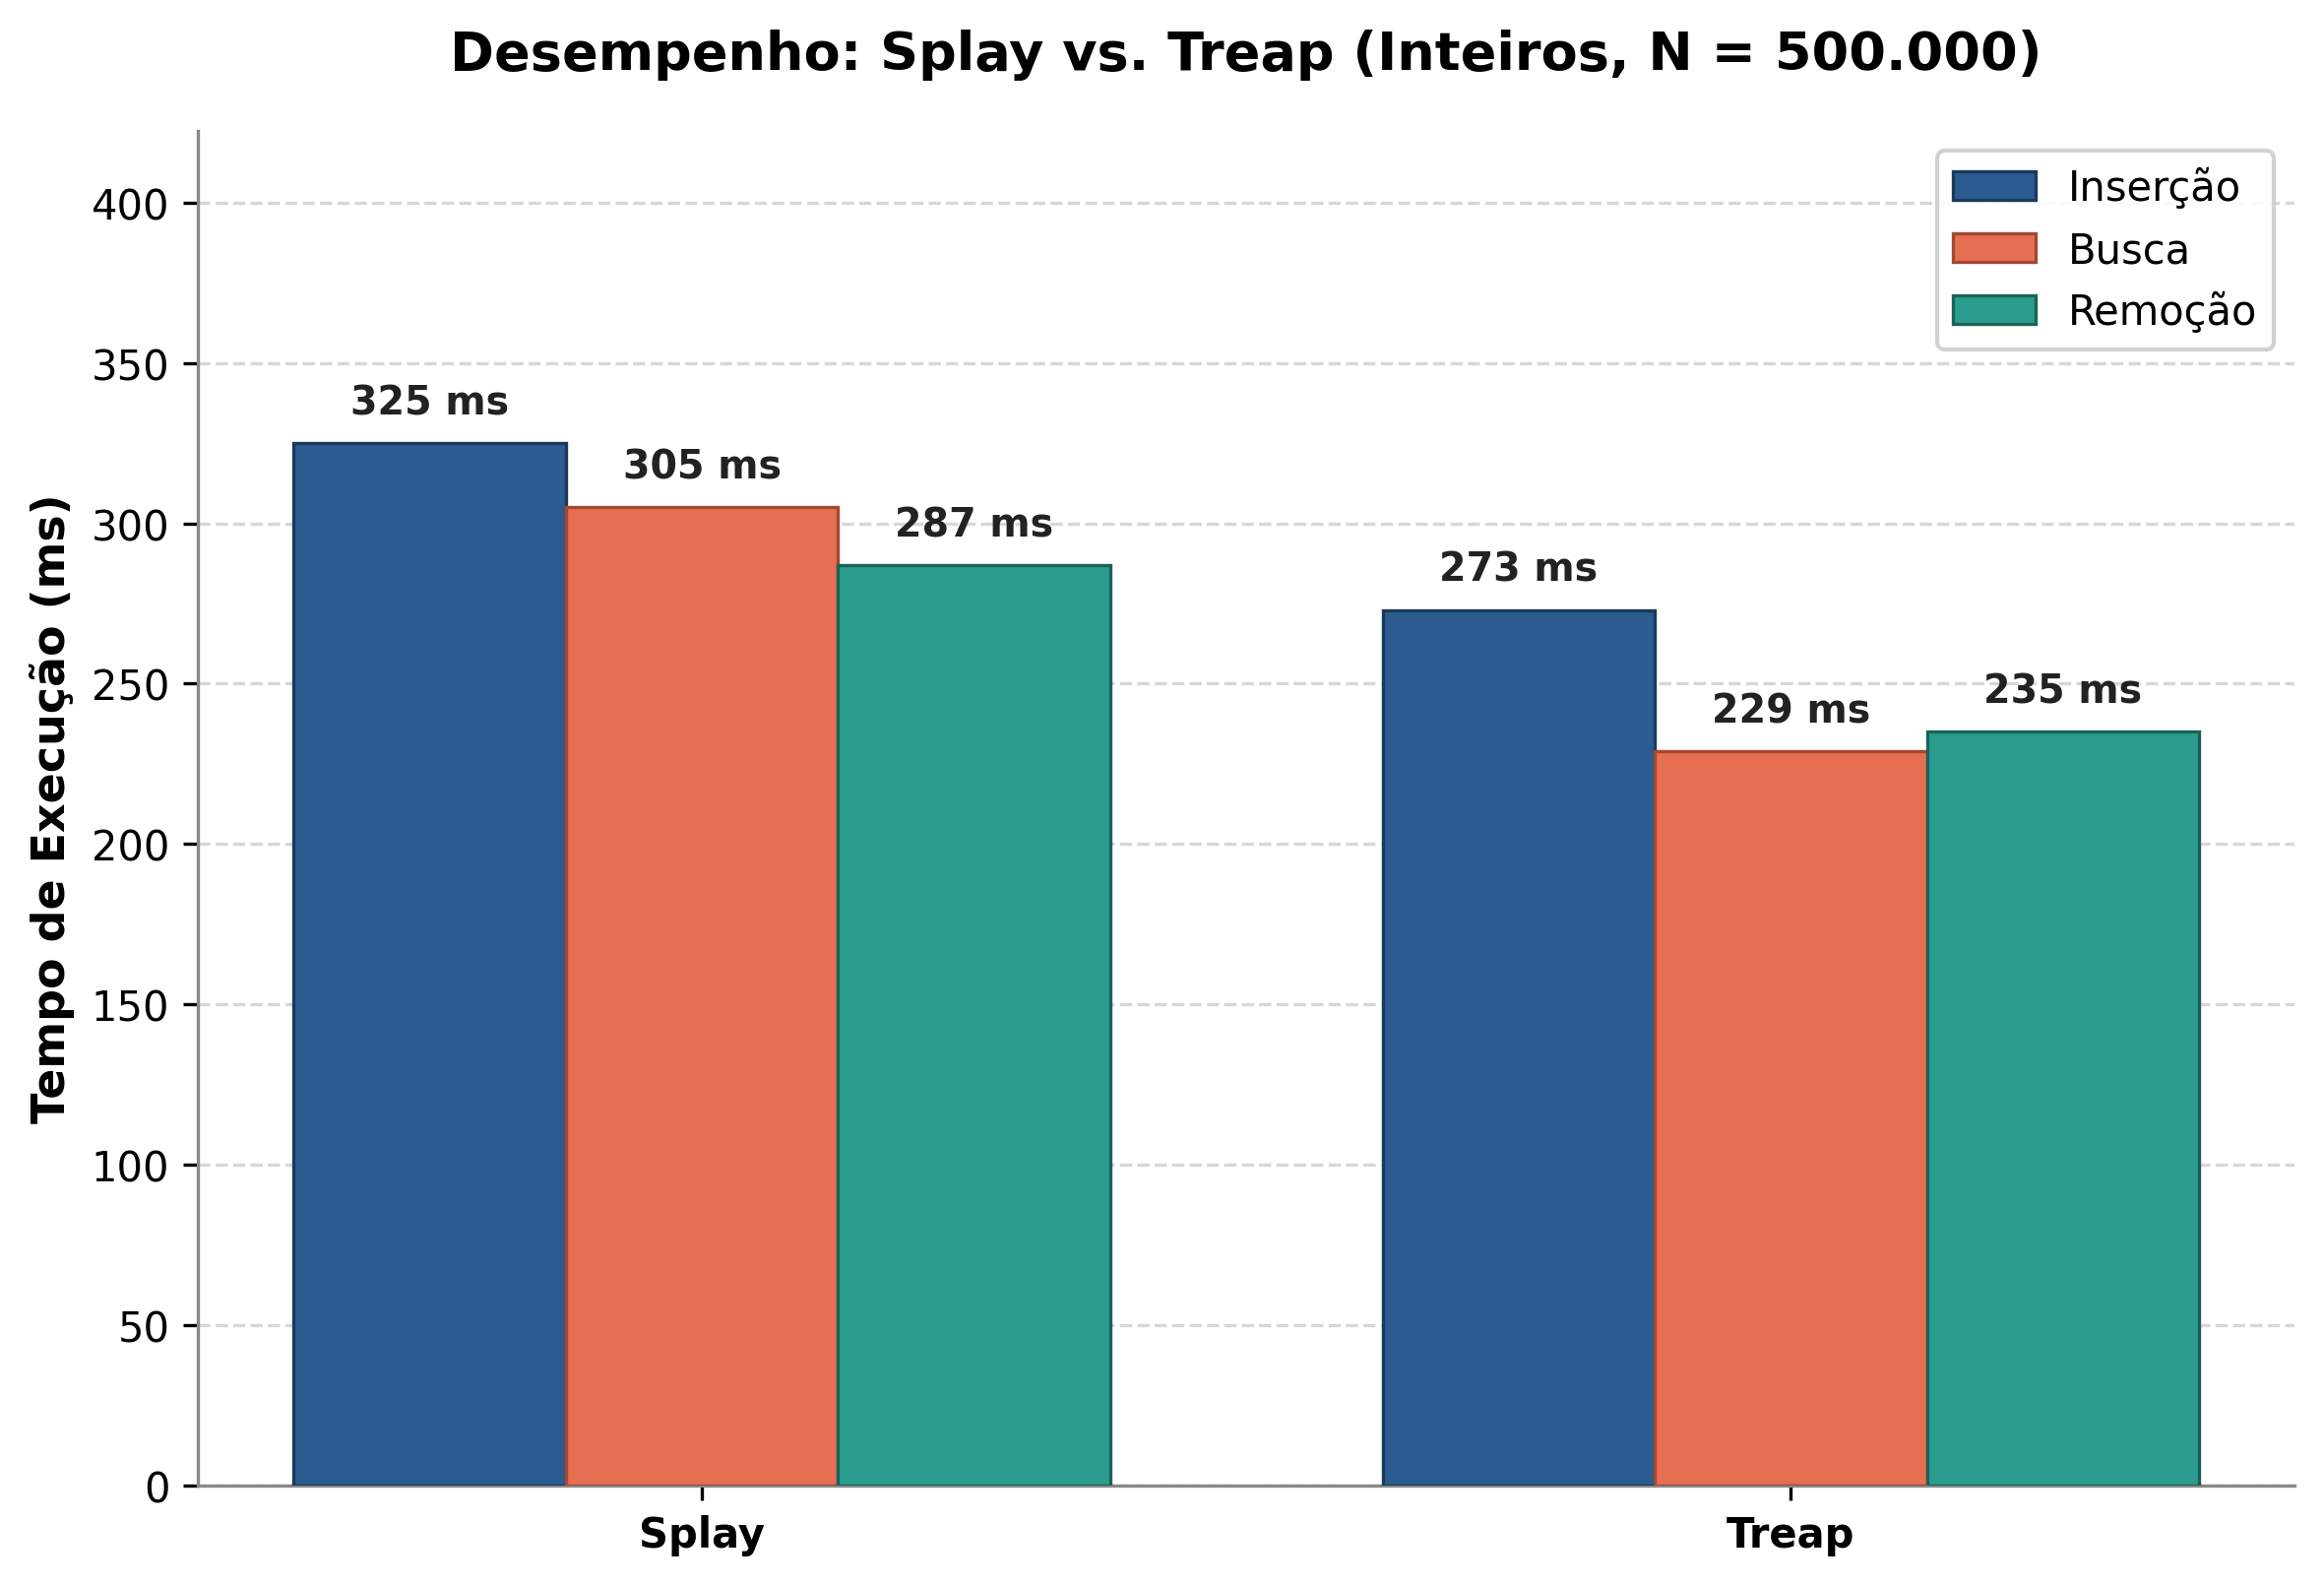
\includegraphics[width=\textwidth]{graficos/benchmark_inteiros.png}
        \caption{Splay vs Treap}
    \end{subfigure}
    \par\medskip
    \begin{subfigure}[b]{0.56\textwidth}
        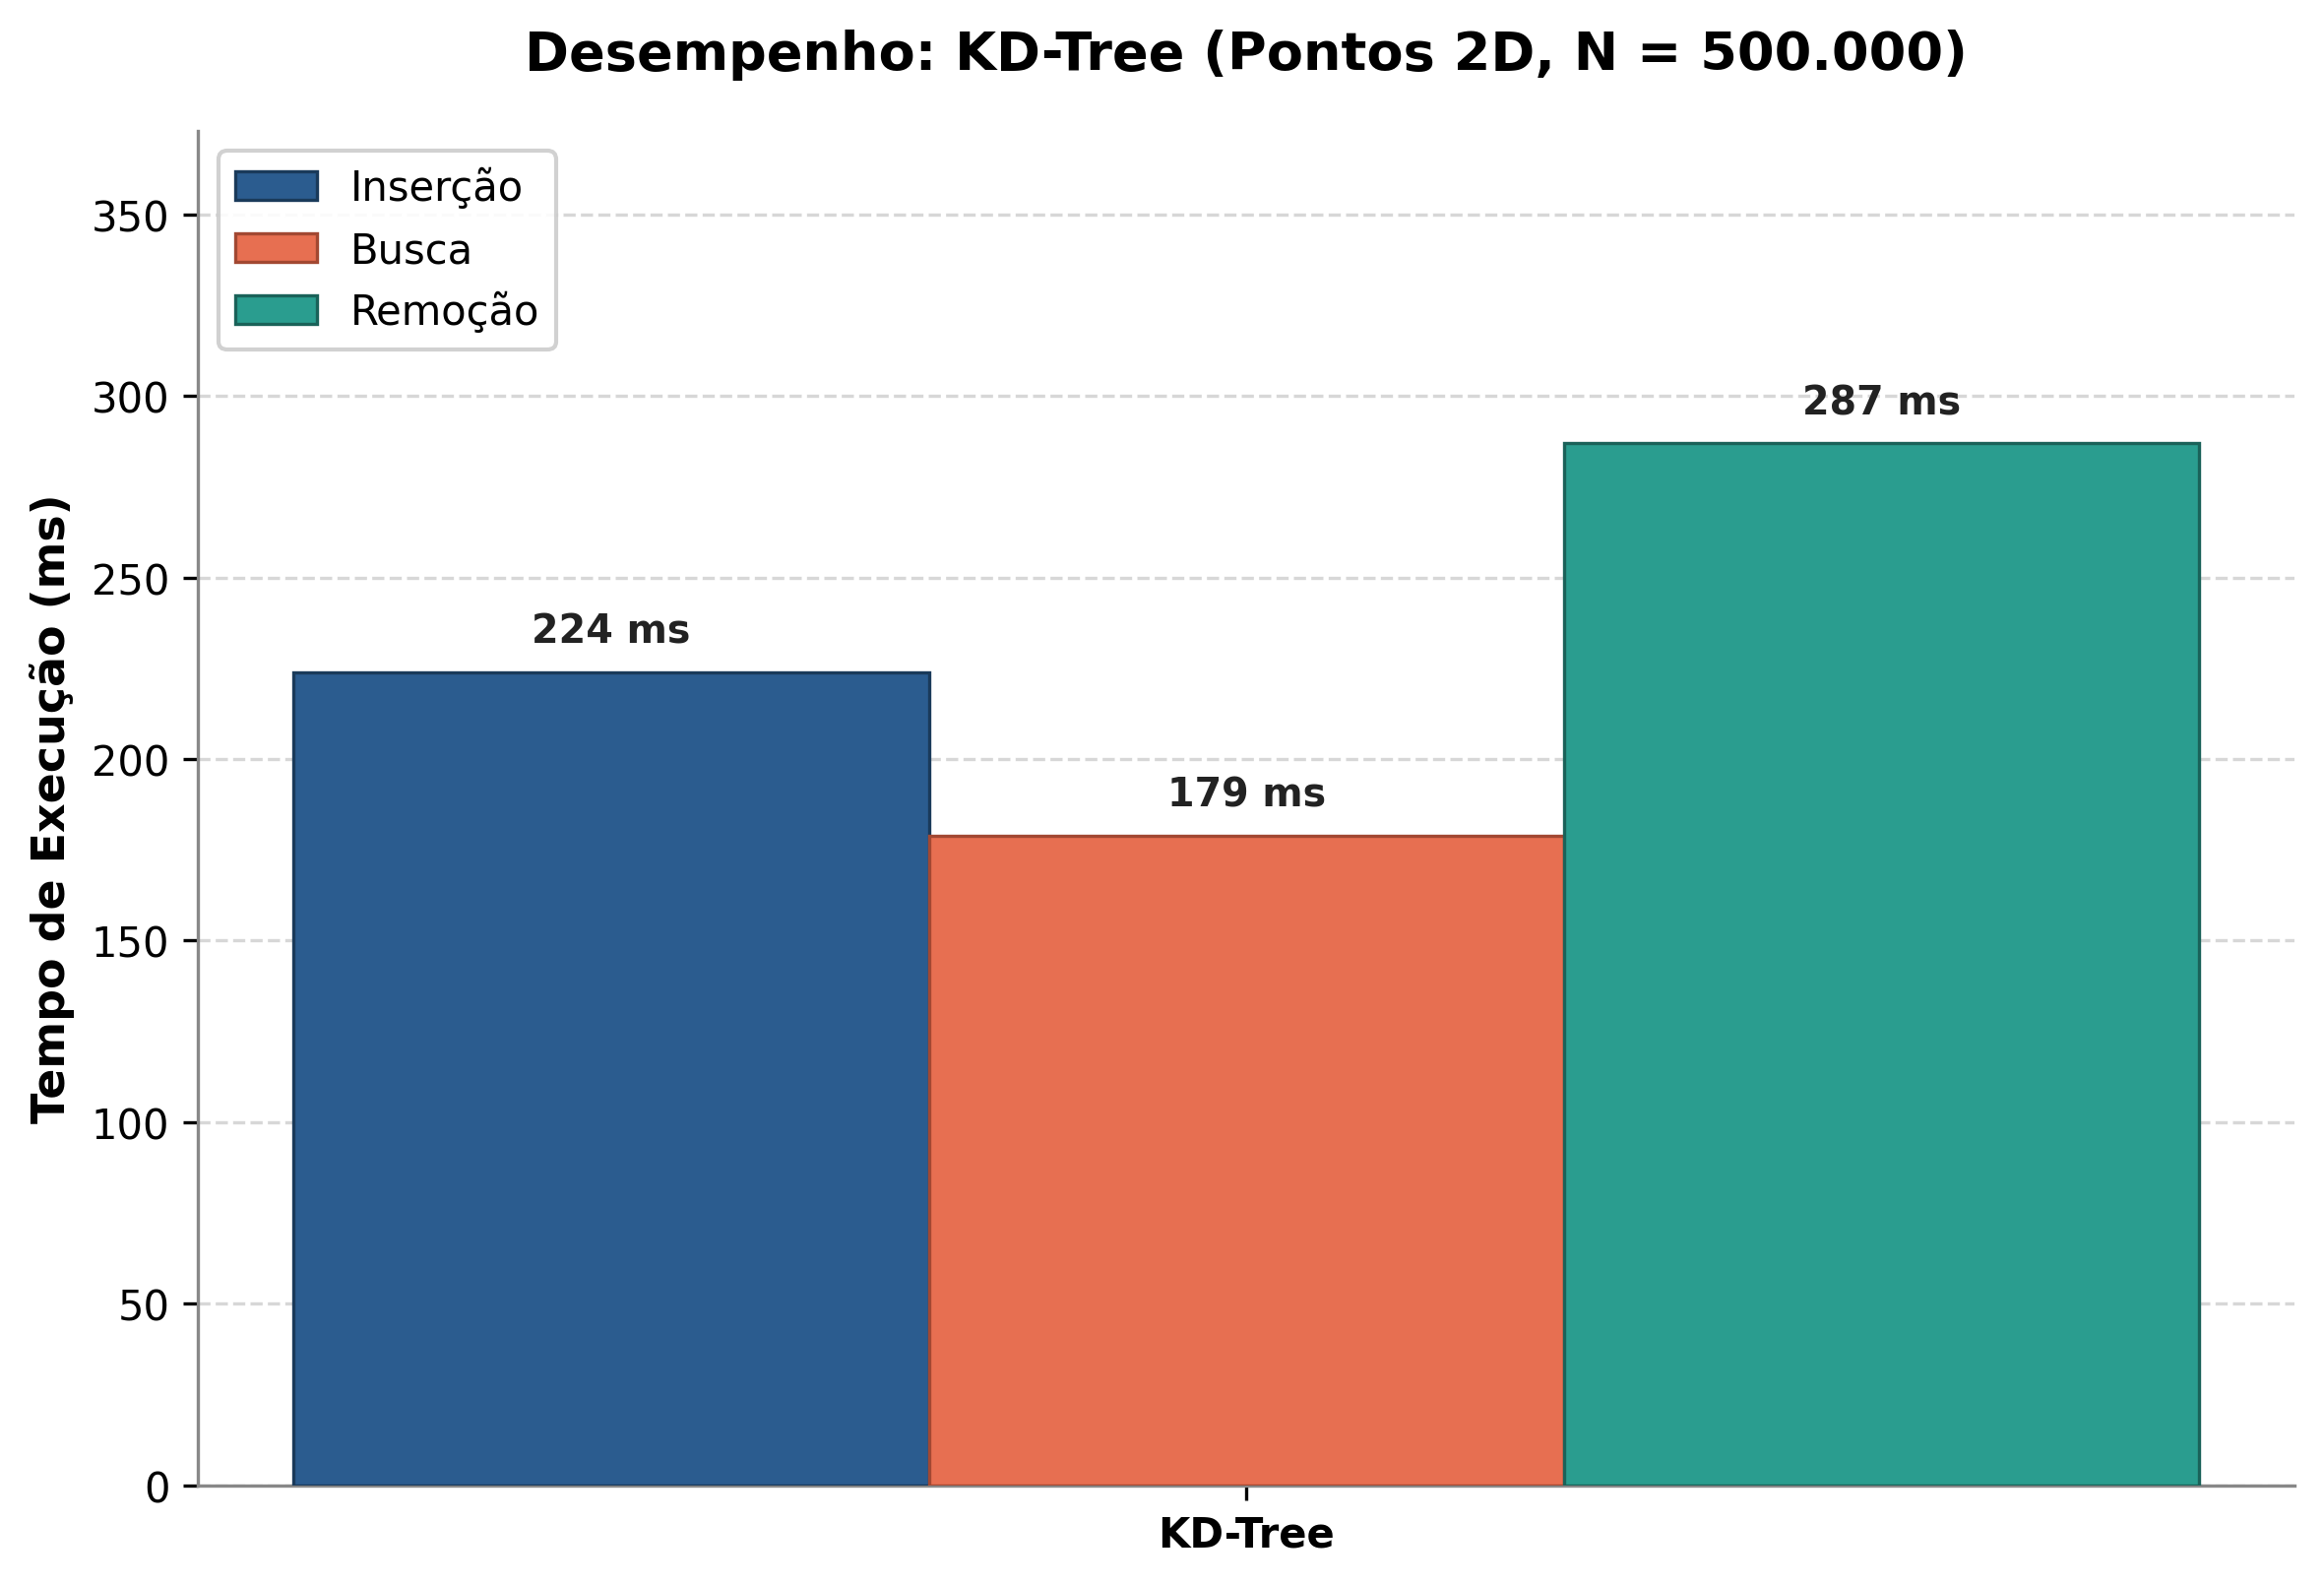
\includegraphics[width=\textwidth]{graficos/benchmark_kdtree.png}
        \caption{KD-Tree}
    \end{subfigure}
    \caption{Desempenho para $N=500\,000$ (mesmos valores da Tabela~\ref{tab:dados_benchmark}).}
    \label{fig:graficos_benchmarks}
\end{figure}

\begin{figure}[H]
    \centering
    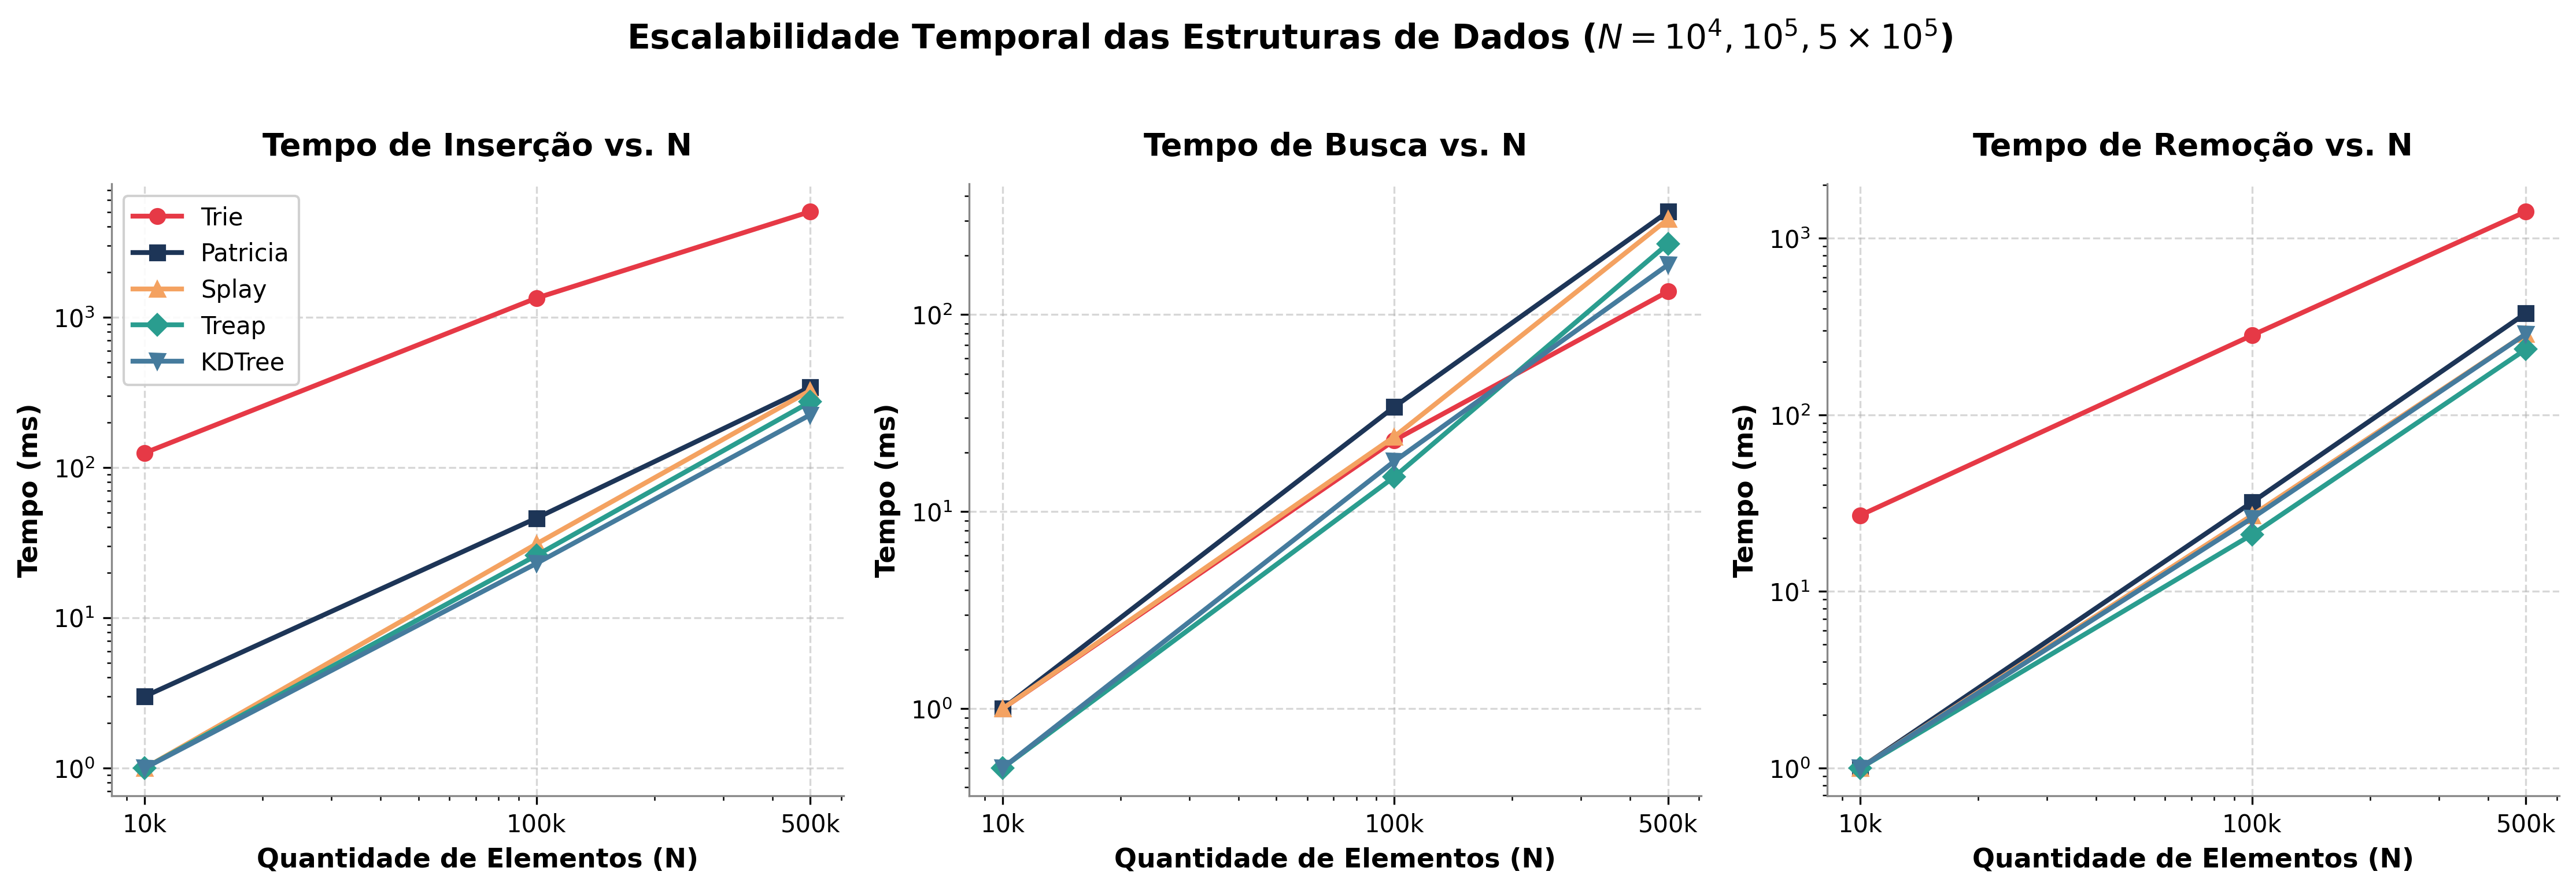
\includegraphics[width=0.96\textwidth]{graficos/benchmark_escalabilidade.png}
    \caption{Escalabilidade temporal (eixos log) para os três valores de $N$; medições de 0\,ms são exibidas em 0,5\,ms apenas para viabilizar a escala logarítmica.}
    \label{fig:escalabilidade}
\end{figure}

\subsection{Memória estrutural e outras distribuições}

\begin{table}[htbp]
\centering
\small
\begin{tabular}{@{}lcrr@{}}
\toprule
\textbf{Estrutura} & \textbf{$N$} & \textbf{Nós} & \textbf{Razão Trie/Patricia} \\ \midrule
Trie / Patricia & $10^{4}$ & 73006 / 12740 & $5{,}7\times$ \\
Trie / Patricia & $10^{5}$ & 655512 / 127398 & $5{,}1\times$ \\
Trie / Patricia & $5\cdot10^{5}$ & 3058444 / 659604 & $4{,}6\times$ \\
\bottomrule
\end{tabular}
\caption{Contagem de nós (\texttt{benchmark\_memory.csv}).}
\label{tab:memoria}
\end{table}

Para aferir assimetrias estruturais e temporais, avaliaram-se inserção estritamente ordenada e uma mistura de consultas com localidade 80-20: 80\% das consultas sorteiam chaves no quinto mais frequente e 20\% em todo o conjunto. Esse gerador expressa localidade, mas não constitui uma distribuição de Zipf estrita. Sob inserção crescente, a Splay registra 1\,ms para $10^{5}$ chaves, pois cada novo máximo torna-se raiz. A Treap mantém altura logarítmica esperada, embora preserve pior caso linear. Na carga 80-20, a Treap foi mais rápida que a Splay nesta execução (19\,ms contra 26\,ms), portanto a concentração adotada não produziu vantagem para a auto-organização da Splay.

\begin{table}[htbp]
\centering
\small
\begin{tabular}{@{}llrrr@{}}
\toprule
\textbf{Padrão} & \textbf{Estrutura} & \textbf{$N$} & \textbf{Inserção (ms)} & \textbf{Busca (ms)} \\ \midrule
ordenado & Splay & $10^{4}$ & 0 & 0 \\
ordenado & Treap & $10^{4}$ & 0 & 0 \\
localidade 80-20 & Splay & $10^{4}$ & --- & 1 \\
localidade 80-20 & Treap & $10^{4}$ & --- & 0 \\ \midrule
ordenado & Splay & $10^{5}$ & 1 & 6 \\
ordenado & Treap & $10^{5}$ & 5 & 5 \\
localidade 80-20 & Splay & $10^{5}$ & --- & 26 \\
localidade 80-20 & Treap & $10^{5}$ & --- & 19 \\
\bottomrule
\end{tabular}
\caption{Desempenho sob distribuições alternativas (\texttt{benchmark\_distributions.csv}).}
\label{tab:dist}
\end{table}

\subsection{Confrontação com a teoria}
Na inserção com $N=5\cdot10^{5}$, Patricia (343\,ms) versus Trie (5039\,ms) dá fator $\approx 14{,}7\times$, coerente com a redução de alocações (Tabela~\ref{tab:memoria}). Na busca pura, a Trie foi mais rápida (131\,ms vs 333\,ms): comparações caractere a caractere em matriz indexada vencem varreduras de prefixos em \texttt{string}. Sob inteiros uniformes, a Treap foi mais rápida que a Splay para $N=500.000$ (inserção 273 vs 325\,ms; busca 229 vs 305\,ms), mantendo a mesma ordem de grandeza esperada. A KD-Tree remove mais caro que busca (287 vs 179\,ms), como previsto pelo \texttt{findMin}. A Splay não dominou o experimento 80-20 medido; a garantia amortizada não implica vantagem de tempo sobre a Treap nessa carga.

\paragraph{Operações espaciais da KD-Tree.}
Os tempos das operações espaciais implementadas, vizinho mais próximo (\texttt{nearestNeighbor}) e busca por faixa (\texttt{rangeSearch}), foram medidos com 10.000 consultas aleatórias em árvores de diversos tamanhos. A Tabela~\ref{tab:kdtree_spatial} apresenta os resultados.

\begin{table}[htbp]
\centering
\small
\begin{tabular}{@{}lcrr@{}}
\toprule
\textbf{Operação} & \textbf{$N$ (árvore)} & \textbf{Consultas} & \textbf{Tempo (ms)} \\ \midrule
Nearest Neighbor & $10^{4}$ & 10.000 & 4 \\
Nearest Neighbor & $10^{5}$ & 10.000 & 10 \\
Nearest Neighbor & $5\cdot10^{5}$ & 10.000 & 15 \\ \midrule
Range Search & $10^{4}$ & 10.000 & 3 \\
Range Search & $10^{5}$ & 10.000 & 13 \\
Range Search & $5\cdot10^{5}$ & 10.000 & 81 \\
\bottomrule
\end{tabular}
\caption{Desempenho das operações espaciais da KD-Tree.}
\label{tab:kdtree_spatial}
\end{table}

O crescimento sublinear observado no tempo de NN (4\,ms $\to$ 10\,ms $\to$ 15\,ms) para 10.000 consultas fixas é compatível com a poda espacial, sem constituir prova isolada da complexidade. As faixas têm lado 10.000 em um domínio de lado $10^6$: cobrem 1\% de cada eixo e 0,01\% da área. O aumento de 3\,ms para 81\,ms reflete tanto a travessia quanto o crescimento de $k$ com $N$.

\section{Aplicações, Análise Crítica e Discussão}

As propriedades estruturais e operacionais observadas ao longo da investigação definem domínios preferenciais de aplicação prática para cada uma das estruturas analisadas:

\begin{itemize}
    \item \textbf{Trie:} Projetada para sistemas de preenchimento automático (\textit{autocomplete}), corretores ortográficos, dicionários de busca textual e analisadores léxicos em compiladores. A capacidade de realizar buscas por prefixo em tempo estritamente proporcional ao comprimento da chave ($O(m)$), independentemente do número de registros armazenados, sobrepuja a dependência logarítmica de árvores binárias convencionais.
    \item \textbf{Patricia (Radix Tree):} Amplamente empregada no encaminhamento de pacotes em redes de computadores, particularmente no algoritmo de casamento de prefixo mais longo (\textit{longest prefix match} em tabelas de roteamento BGP/CIDR), índices invertidos em motores de busca e estruturas de dados de compressão textual. A compactação de caminhos atenua significativamente o consumo de memória frente à Trie comum ao eliminar nós intermediários unários.
    \item \textbf{Splay:} Ideal para implementação de memórias \textit{cache} de software (como tabelas de tradução de endereços virtuais, caches DNS e registros de sessões web) e em cenários caracterizados por forte localidade temporal ou distribuições de acesso enviesadas (distribuição de Zipf). As chaves consultadas com frequência convergem naturalmente para o topo da hierarquia, proporcionando tempos de acesso ultra-rápidos sem sobrecarga de metadados estáticos de balanceamento.
    \item \textbf{Treap:} Estrutura indicada para tabelas de símbolos de uso geral, conjuntos dinâmicos ordenados com alta taxa de mutação e árvores de busca persistentes ou com suporte a operações intervalares (\textit{split} e \textit{merge}). A aleatorização das prioridades torna a altura logarítmica em esperança, independentemente da ordem de entrada, mas não elimina o pior caso linear.
    \item \textbf{KD-Tree:} Padrão fundamental em Sistemas de Informação Geográfica (GIS), algoritmos de agrupamento e vizinhos mais próximos ($k$-NN) em aprendizado de máquina, detecção de colisões espaciais e renderização. A alternância dos eixos particiona o espaço; o balanceamento depende da ordem de inserção ou de uma construção por medianas. Nesta implementação, \texttt{nearestNeighbor} e \texttt{rangeSearch} demonstram a poda espacial.
\end{itemize}

\begin{table}[htbp]
\centering
\scriptsize
\begin{tabular}{@{}l>{\raggedright\arraybackslash}p{6.6cm}>{\raggedright\arraybackslash}p{6.6cm}@{}}
\toprule
\textbf{Estrutura} & \textbf{Vantagens Observadas} & \textbf{Limitações e Riscos Técnicos} \\ \midrule
Trie & Busca por prefixo em tempo $O(m)$; indexação direta em vetor estático de ponteiros sem colisões. & Alto consumo de memória (256 ponteiros: 2048\,B; nó: 2056\,B no ABI verificado); ineficiente para chaves esparsas. \\ \addlinespace
Patricia & Economia expressiva de nós via compressão de caminhos (fator até $5{,}7\times$); inserção acelerada em grandes volumes. & Lógica elaborada de cisão (\textit{split}) e fusão (\textit{merge}); custo de busca ligeiramente superior devido a operações de substring. \\ \addlinespace
Splay & Ausência de metadados de balanceamento; auto-organização dinâmica favorável a padrões de acesso com localidade. & Pior caso individual $O(n)$; operações de busca provocam escritas em memória (mutações topológicas), inviabilizando leituras puras concorrentes. \\ \addlinespace
Treap & Complexidade $O(\log n)$ esperada com balanceamento probabilístico robusto; algoritmos de rotação concisos. & Custo de geração pseudoaleatória de prioridades; campo adicional de 4 bytes, absorvido pelo padding no ABI verificado. \\ \addlinespace
KD-Tree & Busca exata, vizinho mais próximo (\texttt{nearestNeighbor}) e busca por faixa (\texttt{rangeSearch}) em espaço ortogonal com poda eficiente. & Remoção complexa e custosa (\textit{findMin} multidimensional); degradação de desempenho em altas dimensões (maldição da dimensionalidade). \\
\bottomrule
\end{tabular}
\caption{Síntese comparativa de vantagens, limitações e compromissos de projeto.}
\label{tab:tradeoffs}
\end{table}

\subsection{Dificuldades de implementação e reflexão crítica}

Durante a fase de desenvolvimento, a implementação da remoção na KD-Tree representou o maior desafio algorítmico. Quando o nó a ser excluído não possui filho direito, mas possui subárvore esquerda não nula, a substituição pelo predecessor imediato habitual de uma BST unidimensional viola a invariante espacial dos eixos subsequentes. A solução exigiu localizar o nó mínimo ao longo da dimensão de corte corrente na subárvore esquerda via \texttt{findMin}, atribuir suas coordenadas ao nó corrente e migrar recursivamente a subárvore esquerda para o ramo direito (\texttt{root.right =}\allowbreak \texttt{removeHelper(root.left,}\allowbreak \texttt{min.point, depth+1)}), anulando o apontador esquerdo. Além da remoção, a implementação das operações espaciais \texttt{nearestNeighbor} e \texttt{rangeSearch} exigiu a construção cuidadosa da lógica de poda: no vizinho mais próximo, a condição $\mathrm{diff}^2 < \mathrm{bestDist}$ determina se o lado oposto do hiperplano deve ser explorado; na busca por faixa, a interseção do retângulo com o semi-espaço do nó governa a descida.

Na Árvore Patricia, o gerenciamento de substrings durante o \textit{split} de nós intermediários e a subsequente fusão (\textit{merge}) após remoções exigiram rigor extremo no cálculo de comprimentos comuns (\texttt{common\-Prefix\-Length}), evitando a propagação de nós órfãos ou duplicatas lógicas. Já na Árvore Splay, o correto encadeamento das rotações compostas Zig-Zig e Zag-Zag, em que o nó avô deve obrigatoriamente ser rotacionado antes do nó pai, revelou-se determinante para satisfazer o potencial amortizado de Sleator e Tarjan.

Como melhorias futuras, sugerem-se: (i) representação adaptativa de filhos na Trie com tabelas hash esparsas ou arrays comprimidos para alfabetos arbitrários; (ii) construção balanceada estática da KD-Tree baseada em cálculo de medianas no tempo $O(N \log N)$; (iii) extensão da Treap para suportar operações implícitas de concatenação e partição de sequências; e (iv) implementação de $k$-NN (k vizinhos) com fila de prioridade na KD-Tree.

\section{Conclusão}
\label{sec:conclusao}

Este trabalho consolidou a modelagem formal, implementação e experimentação empírica de cinco famílias de árvores computacionais avançadas. A síntese das constatações teóricas e práticas é articulada nas respostas às questões diretivas a seguir:

\paragraph{1. Principais diferenças estruturais entre as abordagens.}
A Trie e a Árvore Patricia organizam dados como árvores digitais sobre sequências alfanuméricas, com ramificações determinadas pelos símbolos constituintes da chave. A Patricia diferencia-se por colapsar nós unários intermediários em arestas compostas, reduzindo drasticamente a quantidade de nós alocados. Em contraste, a Splay e a Treap operam sobre chaves escalares sob a invariante de ordem simétrica de Árvores Binárias de Busca, divergindo na disciplina de balanceamento: a Splay adapta-se deterministicamente a cada acesso via rotações locais que aproximam nós consultados da raiz, enquanto a Treap recorre a prioridades inteiras pseudoaleatórias e rotações de Max-Heap para assegurar altura logarítmica esperada sem depender da ordem das chaves. Por fim, a KD-Tree estende a partição binária para espaços euclidianos $K$-dimensionais alternando ciclicamente o eixo ortogonal discriminante a cada nível da hierarquia.

\paragraph{2. Desempenho empírico por classe de operação e conjunto de dados.}
Na manipulação de strings em larga escala ($N = 500.000$), a Árvore Patricia registrou inserção de 343\,ms contra 5039\,ms da Trie e remoção de 376\,ms contra 1415\,ms, fruto da economia de alocações. A Trie foi mais rápida na busca exata (131\,ms contra 333\,ms). No domínio de inteiros uniformes, a Treap superou a Splay nas três operações medidas. Sob inserção ordenada, a Splay assimilou $100.000$ chaves em 1\,ms. Na KD-Tree, meio milhão de pontos produziram 179\,ms em busca exata e 224\,ms em inserção; 10.000 consultas de vizinho mais próximo consumiram 15\,ms, e 10.000 faixas cobrindo 0,01\% da área levaram 81\,ms.

\paragraph{3. Coerência entre a teoria de complexidade e os dados experimentais.}
Os dados foram coerentes com as tendências teóricas, mas não bastam para identificar expoentes assintóticos com precisão. Trie e Patricia processaram $N$ chaves de comprimento limitado, de modo que o tempo total cresceu aproximadamente com o volume de entrada; a contagem de nós evidenciou a economia estrutural da Patricia. Splay, Treap e KD-Tree apresentaram crescimento compatível com casos médios sublineares por operação, sem excluir seus piores casos lineares. Na carga de localidade 80-20, a Treap registrou 19\,ms contra 26\,ms da Splay, mostrando que a concentração adotada não foi suficiente para produzir vantagem mensurável da auto-organização.

\paragraph{4. Dificuldade de desenvolvimento e aspectos críticos de projeto.}
A KD-Tree e a Árvore Patricia demandaram o maior esforço de implementação. Na KD-Tree, a rotina de remoção impôs o tratamento rigoroso da alternância dimensional e a substituição estrutural pelo mínimo da subárvore esquerda em caso de filho direito nulo, sob pena de violar a invariante geométrica dos eixos subsequentes. Na Patricia, a gerência de cortes e junções de prefixos com atualização precisa de nós terminais exigiu bateria exaustiva de testes para prevenir corrupção topológica. Em contrapartida, a Treap destacou-se pela menor complexidade de código: combinando inserção clássica de BST com rotações locais de Max-Heap no retorno da recursão, assegurou garantias assintóticas robustas com implementação compacta.

\paragraph{5. Diretrizes de escolha para cenários práticos.}
Recomenda-se a Patricia para dicionários volumosos com alta taxa de compartilhamento de prefixos e sistemas de encaminhamento de pacotes sob restrição de memória; a Trie para vocabulários com alfabetos restritos onde a latência mínima de busca é crítica; a Splay para camadas de cache de software, tradução de endereços e cargas com forte viés de acesso temporal; a Treap para coleções dinâmicas de propósito geral que exijam proteção contra entradas adversariais ordenadas sem a sobrecarga de manutenção de árvores Rubro-Negras; e a KD-Tree para indexação espacial e consultas de proximidade euclidiana em dimensões moderadas ($K \le 10$).

\paragraph{6. Síntese comparativa de vantagens e limitações.}
Conclui-se que nenhuma estrutura domina universalmente todos os cenários. A seleção adequada decorre de compromissos técnicos entre ocupação de memória física, custo computacional de rebalanceamento, complexidade de implementação e as distribuições estatísticas das entradas. A compreensão aprofundada das relações entre topologia, análise assintótica e custos reais de arquitetura constitui pré-requisito indispensável para a engenharia de software de alto desempenho.

\subsection*{Disponibilidade de Código e Reprodutibilidade}
\label{sec:repositorio}
O código-fonte integral, testes automatizados, rotinas de compilação e dados experimentais encontram-se disponíveis publicamente no GitHub (\url{https://github.com/HeitorHenriqueZ/Trabalho_Arvores}), suportando: \texttt{make} (compilação com \texttt{-std=c++17 -Wall -Wextra -pedantic}), \texttt{make test} e \texttt{make asan} (testes de corretude e validação via AddressSanitizer), \texttt{make run} (execução de experimentos com persistência em \texttt{data/}) e scripts de análise em \texttt{tools/}.

\begin{thebibliography}{9}
\small
\setlength{\itemsep}{0pt}
\setlength{\parskip}{0pt}
\bibitem{bentley1975}
BENTLEY, Jon Louis. Multidimensional binary search trees used for associative searching. \textit{Communications of the ACM}, v.~18, n.~9, p.~509--517, 1975.
\bibitem{cormen2009}
CORMEN, Thomas H. et al. \textit{Introduction to Algorithms}. 3.~ed. Cambridge: MIT Press, 2009.
\bibitem{fredkin1960}
FREDKIN, Edward. Trie memory. \textit{Communications of the ACM}, v.~3, n.~9, p.~490--499, 1960.
\bibitem{morrison1968}
MORRISON, Donald R. PATRICIA. \textit{Journal of the ACM}, v.~15, n.~4, p.~514--534, 1968.
\bibitem{sedgewick2011}
SEDGEWICK, Robert; WAYNE, Kevin. \textit{Algorithms}. 4.~ed. Boston: Addison-Wesley, 2011.
\bibitem{seidel1996}
SEIDEL, Raimund; ARAGON, Cecilia R. Randomized search trees. \textit{Algorithmica}, v.~16, n.~4, p.~464--497, 1996.
\bibitem{sleator1985}
SLEATOR, Daniel D.; TARJAN, Robert E. Self-adjusting binary search trees. \textit{Journal of the ACM}, v.~32, n.~3, p.~652--686, 1985.
\bibitem{repositorio}
ZONHO, Heitor Henrique. \textit{Trabalho de Árvores Avançadas: Implementação e Avaliação Experimental}. Repositório no GitHub, 2026. Disponível em: \url{https://github.com/HeitorHenriqueZ/Trabalho_Arvores}.
\end{thebibliography}

\end{document}
